\documentclass[11pt]{ubs}
\usepackage{graphicx}
\usepackage{tabularx}
\graphicspath{{figures/}}
\issue{Подготовлено к подаче}
\rubric{Математическая теория управления}
\udk{УДК 004.8}
\bbk{ББК 32.813}

\title{Ландшафтная мера параметрических моделей машинного обучения:
динамика геометрии при обучении}
\engtitle{Landscape Complexity Measure of Models: Dynamics of Loss Geometry During Training}

\authors{
\textbf{Грабовой~А.В.}\footnote{Андрей Валериевич Грабовой, к.ф.-м.н., с.н.с. \emph{(}grabovoy@ipu.ru\emph{)}.}\\
\textit{\emph{(}ФГБУН Институт проблем управления им.~В.А.~Трапезникова РАН, Москва\emph{)}}
}

\engauthors{
\textbf{Andrey Grabovoy}, Institute of Control Sciences of RAS, Moscow,
Candidate of Sciences (Physics and Mathematics), Senior Researcher (grabovoy@ipu.ru).}

\abstract{
Современные исследования больших языковых моделей описывают качество через число параметров, объем данных и вычислительный бюджет, описывая геометрию функции потерь преимущественно качественным анализом.
В данной работе количественно анализируется динамика ландшафтной меры как среднего разброса матриц Гессе по объектам обучения вдоль траектории оптимизации языковых нейросетевых моделей и ее связь с ошибкой на валидационной выборке.
Мера задает компактную характеристику локальной неоднородности ландшафта и дополняет показатели качества сведениями о геометрии ландшафта, причем численное значение опирается на малую подвыборку контекстов и сравнение гессианов по спектральной норме с пересэмплированием на контрольных точках, поэтому отражает выборочную локальную информацию, а не полный набор свойств модели.
В работе показано, что траектория меры в общем случае не сводится к траектории ошибки, а именно при монотонном улучшении ошибки мера может вести себя немонотонно, в том числе возрастая на поздних участках обучения.
На совместной диаграмме валидационной ошибки и меры одному уровню ошибки соответствуют различные значения меры в зависимости от этапа обучения и архитектуры.
Простая линейная связь меры с ошибкой и логарифмом объема обучения оставляет заметные остатки во второй части эксперимента и при сравнении различных архитектурных конфигураций.
}

\engabstract{
Empirical studies of large language models typically report performance via parameter count, data volume, and compute budget, whereas loss-landscape geometry is still discussed mainly at a qualitative level.
This work quantifies the dynamics of a landscape measure~---the average dispersion of per-example Hessians along the optimization trajectory for neural language models---and relates it to validation error.
The measure summarizes local heterogeneity of the landscape and complements predictive-quality indicators with geometry-of-risk information; being based on a small probe set and spectral-norm Hessian comparisons, it reflects local sampling-based evidence rather than complete model properties.
The measure trajectory need not track the error trajectory: error can improve monotonically while the measure changes non-monotonically and may rise late in training.
Joint error--measure plots show that equal validation error can accompany different measure values depending on training stage and architecture.
A linear model tying the measure to error and the logarithm of training volume still exhibits sizable residuals on long runs and across architectural variants.
}

\keywords{ландшафтная мера, матрица Гессе, языковые модели, динамика обучения, геометрия функции потерь}
\engkeywords{landscape measure, Hessian, language models, training dynamics, loss geometry}

\presented{...}
\received{...}
\published{...}

\begin{document}

\maketitle

\section{Введение}
Обучение современных больших параметрических моделей глубокого обучения требует все больше вычислительных ресурсов и времени.
В свою очередь качество моделей сильно зависит от архитектуры модели, данных и метода обучения~\cite{kaplan2020,hoffmann2022}.
Перебор архитектур и данных для поиска оптимальной модели требует больших вычислительных затрат, что делает эмпирический анализ качества модели сложным и трудоемким.

Современные направления исследований для поиска оптимальных архитектур моделей нацелены на эмпирические законы масштабирования, связывающие качество, размер модели и объем данных при ограниченном вычислительном бюджете~\cite{kaplan2020,hoffmann2022}.
Анализ опирается на срезы фиксированного бюджета и сопоставление режимов с разным соотношением числа параметров и числа токенов.
Другим направлением анализа моделей глубокого обучения является качественный анализ ландшафта функции потерь и его связи с качеством модели~\cite{choromanska2015,li2018visualizing,fort2019emergent,fort2019large}.
Они опираются на анализ спектра матриц Гессе и его связи с качеством модели.
На основе работ~\cite{kiselev2024,meshkov2024ispras}, где ландшафтная мера сложности вводится в фиксированной точке, в настоящей работе изучается ее динамика вдоль траектории обучения.

Эмпирически фиксируются смены геометрического режима, в том числе резкие изменения ландшафтной меры~$\mu$ при переходах между фазами оптимизации.
Для анализа проводится вычислительный эксперимент на модели GPT-2~\cite{radford2019language} с различным числом параметров и объемом обучающих данных на корпусе WikiText-103~\cite{merity2016pointer}.

\section{Связанные работы}\label{sec:related}

Большое число современных исследований посвящено спектральным свойствам матрицы Гессе эмпирического риска и их связи с динамикой оптимизации и организацией ландшафта~\cite{sagun2018,ghorbani2019,papyan2019,pennington2017,wu2022dissecting}.
В эмпирическом анализе переобученных сетей~\cite{sagun2018} изучаются распределения собственных значений матрицы Гессе, где выделяются основная часть спектра и выбросные собственные значения, обсуждается связь этой структуры с ходом градиентного обучения.
Работа~\cite{ghorbani2019} направлена на анализ плотности распределения собственных значений матрицы Гессе.
Данная плотность используется как инструмент анализа оптимизации нейронных сетей в рамках которого получаются количественные характеристики этой плотности в типичных режимах обучения.
В~\cite{papyan2019} анализируется структура спектра матрицы Гессе для крупных моделей глубокого обучения.
В частности показано, как структура спектра соотносится с числом классов и объемом данных.
В работе~\cite{pennington2017} используется аппарат теории случайных матриц для описания геометрии поверхностей потерь нейросетей.
В~\cite{wu2022dissecting} выделяются общие закономерности структуры Гессиана по слоям и типам параметров, то есть анализируется не только спектр одной агрегированной матрицы, но и устойчивые шаблоны внутри архитектуры.

Отдельно исследуется связь обобщения и устойчивости с геометрией минимума около найденного решения~\cite{hochreiter1994,neyshabur2017exploring,dinh2017sharp}.
В классической постановке~\cite{hochreiter1994} плоские области функции потерь интерпретируются как предпочтительные с точки зрения описательной сложности решения и обобщающей способности.
В~\cite{neyshabur2017exploring} систематизируются эмпирические закономерности обобщения в глубоких сетях и анализируется связь качества с режимом оптимизации~\cite{hochreiter1994} и геометрией ландшафта без сведения к одному скалярному показателю неоднородности разброса матриц Гессе между объектами обучения.
В~\cite{dinh2017sharp} показывается, что формулировки про острые минимумы как худшие для обобщения не универсальны.
В частности, приводятся примеры и теоретические конструкции, которые демонстрируют случаи хорошего обобщения при остром минимуме, то есть постановка опирается на чувствительность решения к возмущениям в окрестности минимума, а не на разброс Гессе по обучающим точкам.

Работы~\cite{choromanska2015,li2018visualizing,fort2019emergent,fort2019large} дополняют спектральный анализ качественной картиной организации поверхности потерь.
В~\cite{choromanska2015} анализируется структура поверхностей потерь многослойных сетей и связь качественных свойств ландшафта с упрощенными статистическими моделями.
В~\cite{li2018visualizing} предложены методы снижения размерности и нормировки фильтров для сравнения формы ландшафта между архитектурами и режимами обучения.
В работах~\cite{fort2019emergent,fort2019large} описывается локальная геометрия, связность областей низкой ошибки, пути между решениями и организация бассейнов при разном распределении данных.

Ближайшим к настоящей работе направлением исследованием является ландшафтная мера на основе матриц Гессе по объектам обучения.
В работах~\cite{kiselev2024,meshkov2024ispras} развивается конструкция ландшафтной меры на основе матриц Гессе, сопоставляемых каждому объекту обучения.
Для полносвязных архитектур в задаче классификации в~\cite{kiselev2024} построены спектральные мажоранты и верхние оценки на ландшафтную меру сложности в оптимуме.
В работе~\cite{meshkov2024ispras} проводится обобщение данного подхода для матричных моделей глубокого обучения.
Работа~\cite{petrov2025curvaturegap} посвящена закономерностям кривизны при масштабировании трансформерных моделей.
Работы~\cite{singh2024lmc,singh2022double} анализируют явление двойного спуска и связанные с ним изменения режимов обучения при обучении моделей глубокого обучения.
В режиме предельно широких сетей динамика обучения описывается через нейронного касательного ядра в постановке~\cite{jacot2018ntk} и последующих работах~\cite{lee2018wide}.
В пределе динамика становится линейной в функциональном пространстве относительно фиксированного ядра, что по смыслу отличается от режима сетей конечной ширины и от неоднородности разброса матриц Гессе по объектам, которую отражает ландшафтная мера.

Параллельно изучаются скалярные характеристики кривизны в точке~$\theta$. Рассматривается след матрицы Гессе, максимальное собственное значение, плотность спектра и производные от них~\cite{ghorbani2019,papyan2019,wu2022dissecting,petrov2025curvaturegap}.
Такие величины описывают агрегированную кривизну функции ошибки в окрестности~$\theta$ и дополняют, но не заменяют, показатели межобъектного рассогласования гессианов, вводимых в работе~\cite{kiselev2024}.

\section{Постановка задачи}\label{sec:problem}

Пусть~$\Theta$~--- пространство допустимых значений вектора параметров модели глубокого обучения.
Эмпирические функции потерь на валидационной и обучающей выборках задаются~$\mathcal{L}_{\mathrm{val}}(\theta)$ и~$\mathcal{L}_{\mathrm{train}}(\theta)$ соответственно.

Точку минимума эмпирического риска на обучении обозначим через
\begin{equation}
  \theta^\star \in \arg\min_{\theta\in\Theta} \mathcal{L}_{\mathrm{train}}(\theta).
\end{equation}

Для анализа локальной геометрии эмпирического риска в точке~$\theta\in\Theta$ фиксируется конечное множество
\[
  D_{\mathrm{probe}} = \{x_1,\ldots,x_m\}.
\]
Пусть для каждого объекта~$x_i\in D_{\mathrm{probe}}$ задана~$\mathbf{H}_i(\theta)$~--- матрица Гессе функции~$\ell(\theta;x_i)$ в точке~$\theta$.
Здесь~$x_i$~--- это некоторый токенизированный контекст фиксированной длины~$L_{\mathrm{ctx}}$, тогда функция ошибки для языкового моделирования имеет вид
\[
  \ell(\theta;x_i)= -\frac{1}{L_{\mathrm{ctx}}-1}\sum_{k=1}^{L_{\mathrm{ctx}}-1}\log p_\theta\bigl(x_{i,k+1}\mid x_{i,1:k}\bigr).
\]
Усреднение по объектам из выборки~$D_{\mathrm{probe}}$ вводится следующим образом:
\begin{equation}\label{eq:probe-hessians}
  \mathbf{H}_i(\theta)=\nabla_\theta^2 \ell(\theta;x_i), \qquad
  \bar{\mathbf{H}}(\theta)=\frac{1}{m}\sum_{i=1}^{m}\mathbf{H}_i(\theta),
\end{equation}
Рассмотрим ландшафтную меру, задаваемую выражением:
\begin{equation}\label{eq:mu-def}
  \mu(\theta)=\frac{1}{m}\sum_{i=1}^{m}\left\|\mathbf{H}_i(\theta)-\bar{\mathbf{H}}(\theta)\right\|_2,
\end{equation}
где~$\|\cdot\|_2$~--- спектральная норма матрицы.
Заметим, что при~$\theta=\theta^\star$ величина~$\mu(\theta)$ совпадает с ландшафтной мерой сложности в постановке~\cite{kiselev2024}.

Величина~$\mu$ по смыслу отличается от традиционных скалярных показателей ``остроты'' по спектру агрегированного Гессиана~\cite{ghorbani2019,papyan2019,wu2022dissecting}: последние характеризуют одну матрицу в точке~$\theta$, тогда как~\eqref{eq:mu-def} измеряет разброс семейства~$\{\mathbf{H}_i\}$ между обучающими контекстами.

Рассматривается траектория обучения~$\{\theta_t\}_{t=1}^{T}$, параметризованная неотрицательным накопленным числом токенов~$t$.
Вдоль нее рассматривается пара отображений~$\mathcal{L}_{\mathrm{val}}(\theta_t)$ и~$\mu(\theta_t)$.

Пусть~$\mathcal{T}=\{t_j\}_{j=1}^{J}$~--- множество контрольных значений накопленного числа токенов для соответствующих состояний~---~$\theta_{t_j}$,~$j=1,\ldots,J$.
На этой дискретизации сопоставляются значения~$\mathcal{L}_{\mathrm{val}}(\theta_{t_j})$ и~$\mu(\theta_{t_j})$, анализируется совместная динамика при возрастании~$t_j$.

\section{Вычислительный эксперимент}\label{sec:exp}
\begin{table}[htbp]
\caption{Множество архитектур модели GPT-2 для экспериментального сравнения динамики ландшафтной меры}%
\label{tab:arch-grid}
\centering
\footnotesize
\setlength{\tabcolsep}{3pt}
\begin{tabularx}{\linewidth}{|*{9}{>{\centering\arraybackslash}X|}}
\hline
$L$ & $H$ & $E$ & $L$ & $H$ & $E$ & $L$ & $H$ & $E$ \\
\hline
$2$ & $2$ & $48$ & $2$ & $2$ & $64$ & $2$ & $2$ & $80$ \\
$2$ & $2$ & $96$ & $2$ & $4$ & $112$ & $2$ & $4$ & $128$ \\
$3$ & $2$ & $48$ & $3$ & $2$ & $64$ & $3$ & $2$ & $80$ \\
$3$ & $2$ & $96$ & $3$ & $4$ & $112$ & $3$ & $4$ & $128$ \\
$4$ & $2$ & $48$ & $4$ & $2$ & $64$ & $4$ & $2$ & $80$ \\
$4$ & $2$ & $96$ & $4$ & $4$ & $112$ & $4$ & $4$ & $128$ \\
$5$ & $2$ & $48$ & $5$ & $2$ & $64$ & $5$ & $2$ & $80$ \\
$5$ & $2$ & $96$ & $5$ & $4$ & $112$ & $5$ & $4$ & $128$ \\
$6$ & $2$ & $48$ & $6$ & $2$ & $64$ & $6$ & $2$ & $80$ \\
$6$ & $2$ & $96$ & $6$ & $4$ & $112$ & $6$ & $4$ & $128$ \\
$7$ & $2$ & $48$ & $7$ & $2$ & $64$ & $7$ & $2$ & $80$ \\
$7$ & $2$ & $96$ & $7$ & $4$ & $112$ & $7$ & $4$ & $128$ \\
\hline
\end{tabularx}
\end{table}
\begin{table}[htbp]
\caption{Численные параметры эксперимента}%
\label{tab:exp-params}
\centering
\footnotesize
\setlength{\tabcolsep}{4pt}
\begin{tabularx}{\linewidth}{|p{2.35cm}|>{\raggedright\arraybackslash}X|}
\hline
Параметр & Значение \\
\hline
Данные & WikiText-103~\cite{merity2016pointer}; токенизатор GPT-2~\cite{radford2019language}; длина контекста~$L_{\mathrm{ctx}}=128$ токенов; сетка~$(L,H,E)$ числа слоев, голов и размерности эмбеддинга~--- табл.~\ref{tab:arch-grid} \\
\hline
Первая часть &~$36$ конфигураций; бюджет обучения~$\approx 1{,}2\cdot 10^{7}$ токенов;~$20$ контрольных точек по накопленным обучающим токенам; мини-пакет~$128$ контекстов;~$8$ независимых запусков обучения на архитектуру; AdamW:~$\mathrm{lr}=3\cdot 10^{-4}$, weight decay~$0{,}01$ \\
\hline
Вторая часть & архитектуры~$(2,2,48)$,~$(5,2,96)$,~$(7,4,128)$; бюджет до~$1{,}5\cdot 10^{8}$ токенов;~$36$ контрольных точек; мини-пакет~$128$;~$8$ независимых запусков обучения; AdamW: разогрев~$3\%$ итераций, косинусное снижение~$\mathrm{lr}$ до~$3\cdot 10^{-5}$ \\
\hline
Оценка~$\mu$ & на каждой контрольной точке: новая мини-выборка~$D_{\mathrm{probe}}$ из~$m=8$ контекстов из текущего обучающего потока;~$r=4$ независимых случайных направления для нижней оценки спектральной нормы через гессиан-векторные произведения \\
\hline
\end{tabularx}
\end{table}
\begin{figure}[ht]
\centering
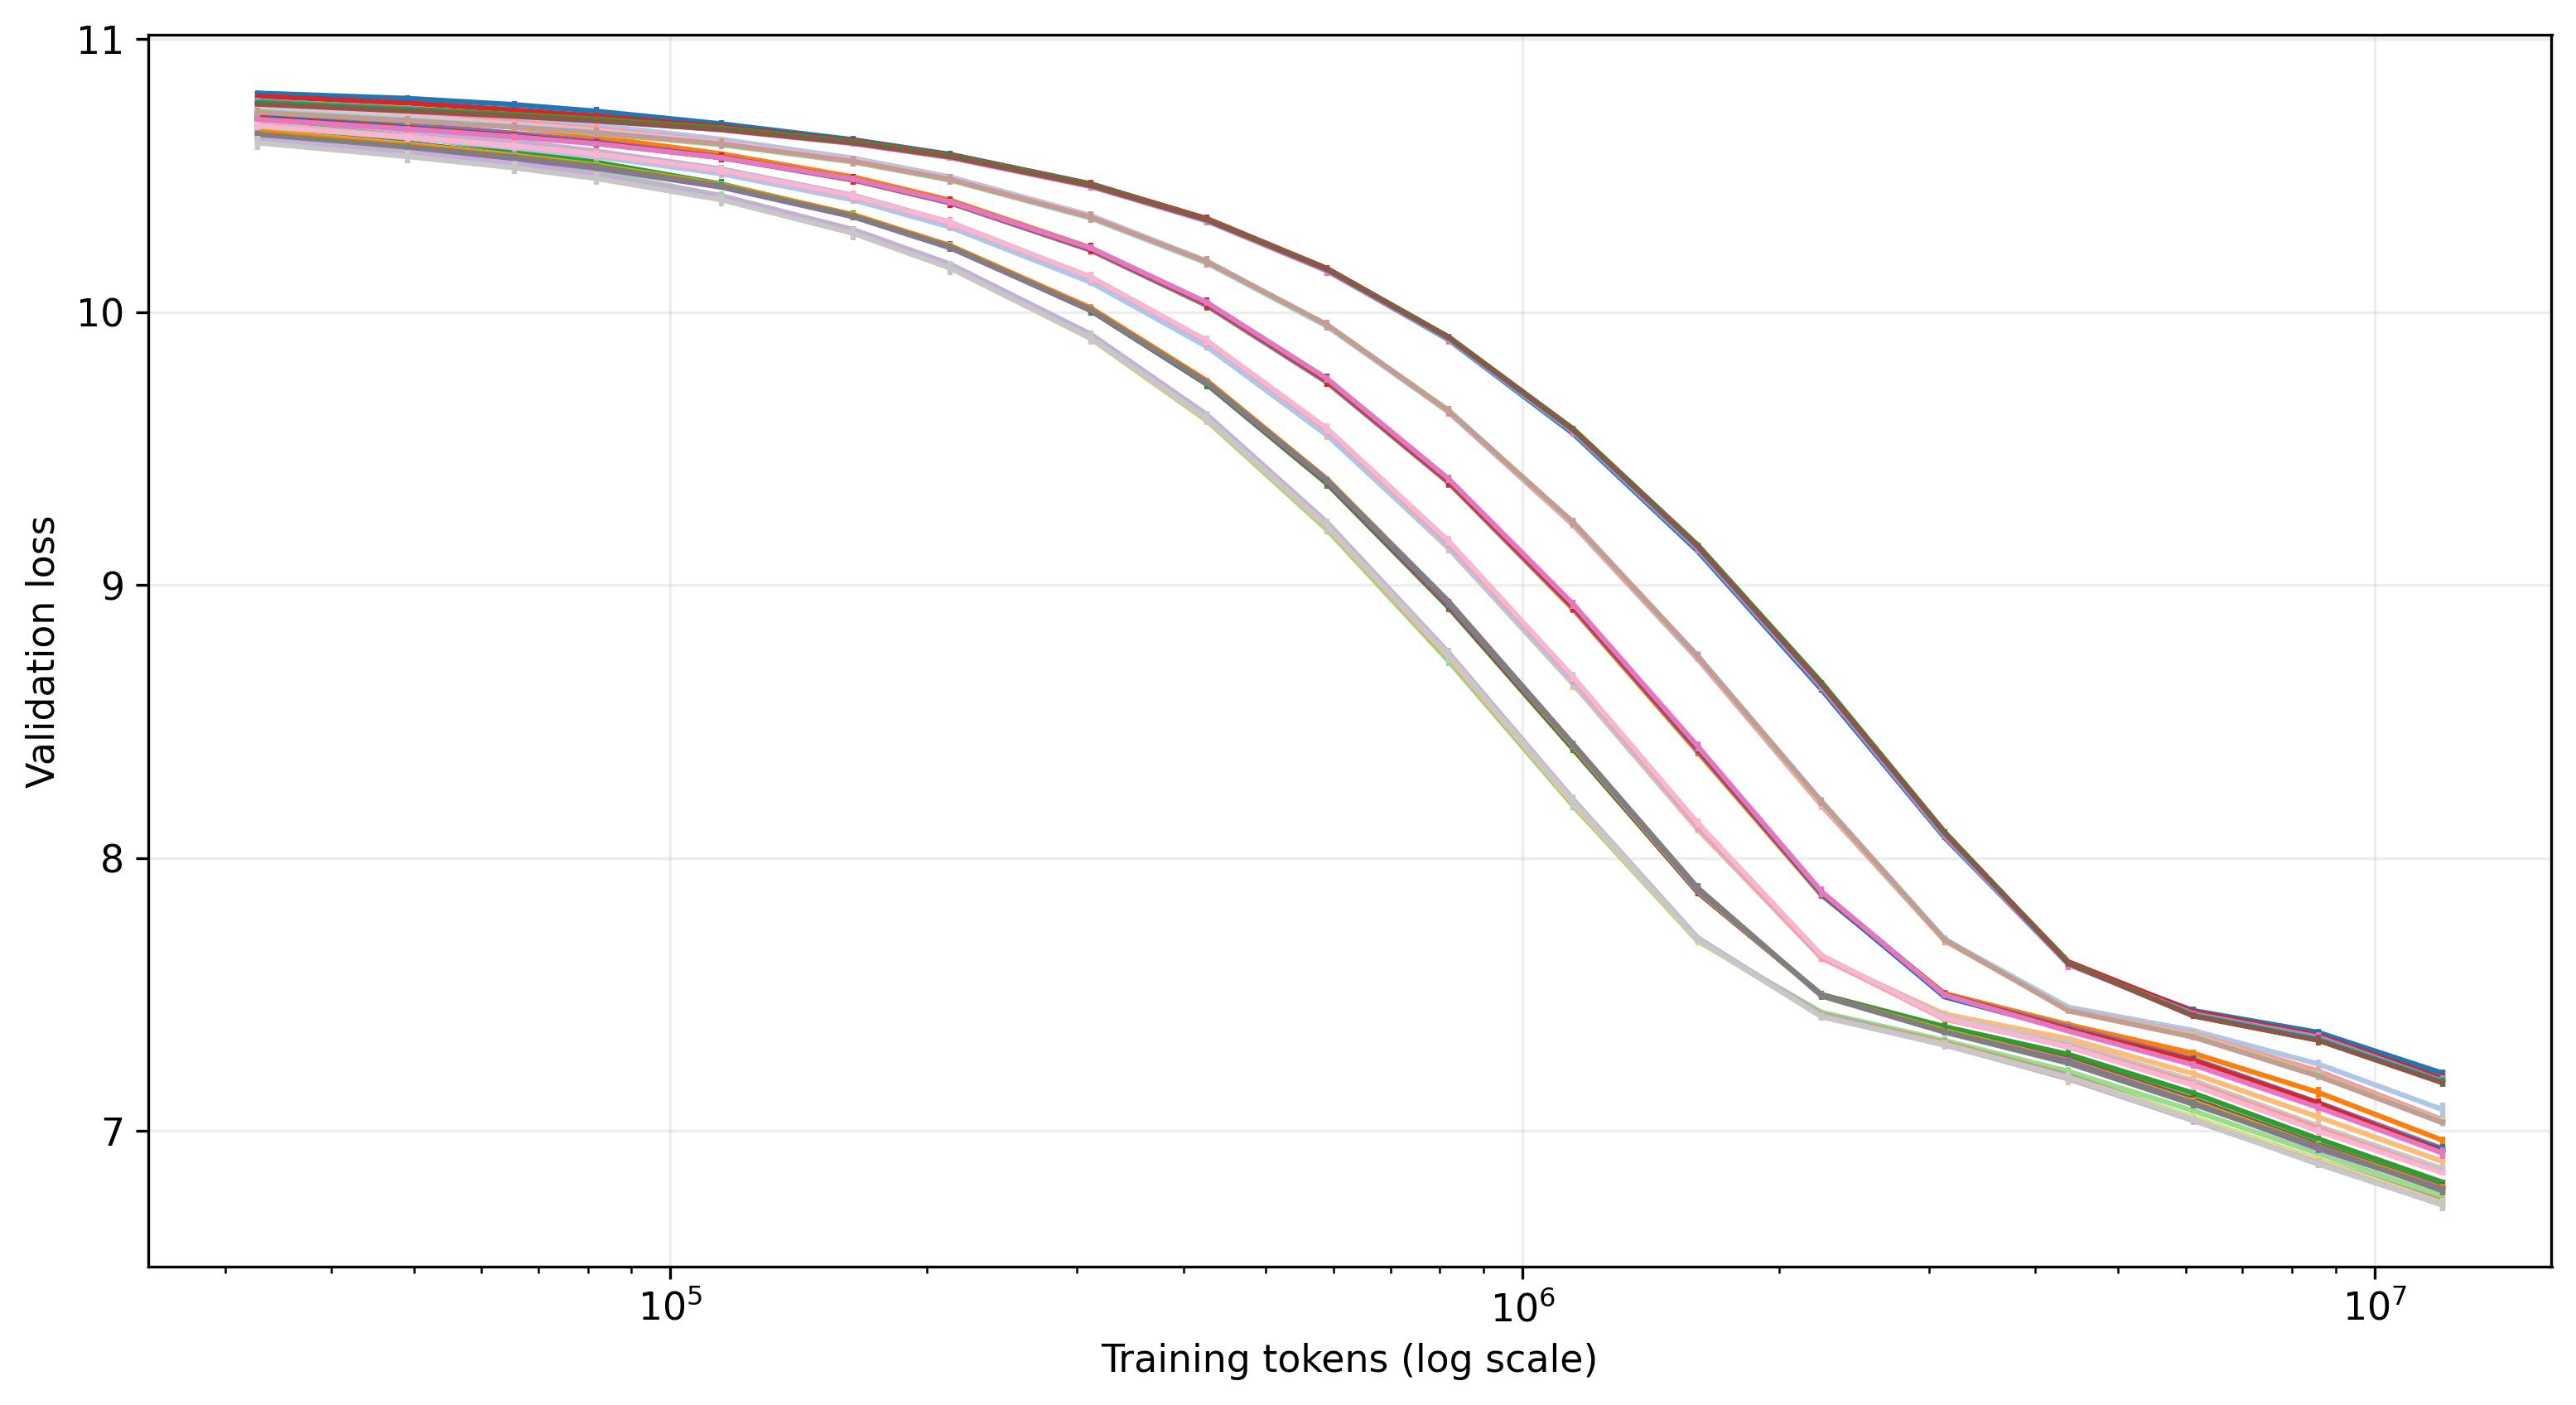
\includegraphics[width=0.92\linewidth]{fig_loss_all_models.png}
\caption{Валидационная ошибка в зависимости от числа обработанных обучающих токенов}
\label{fig:loss-all}
\end{figure}
\begin{figure}[ht]
\centering
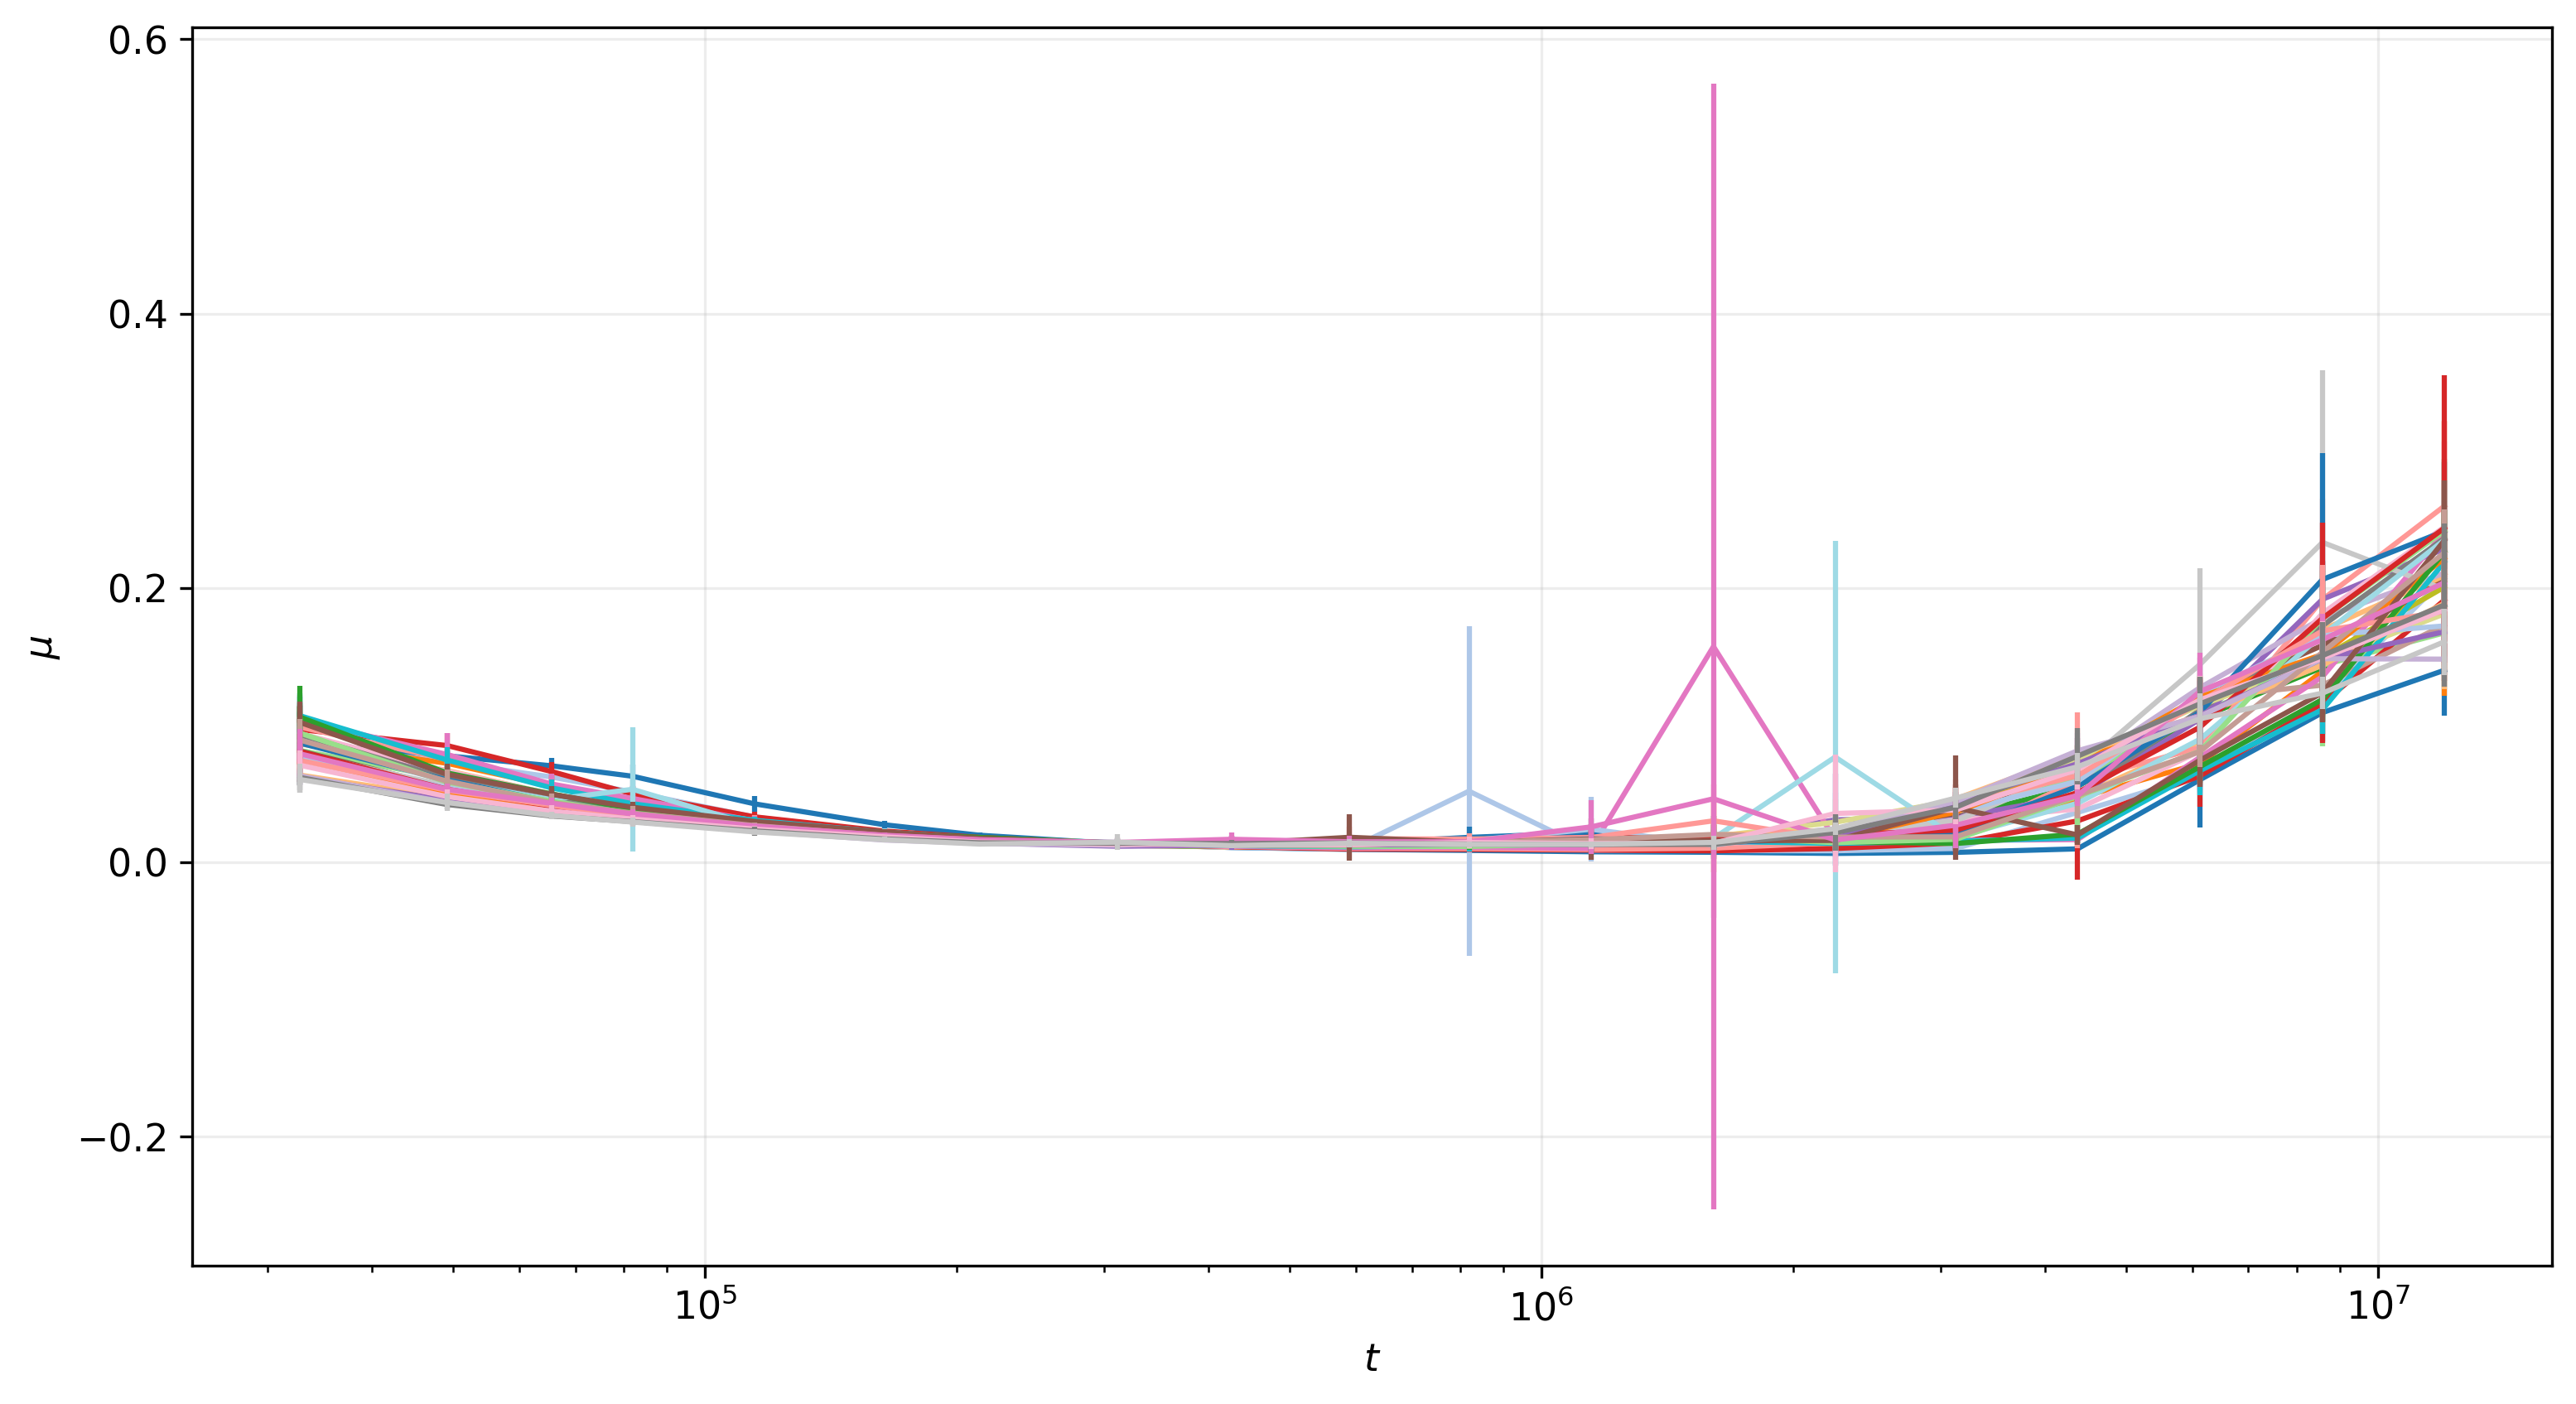
\includegraphics[width=0.92\linewidth]{fig_mu_all_models.png}
\caption{Ландшафтная мера в процессе обучения}
\label{fig:mu-all}
\end{figure}
\begin{figure}[ht]
\centering
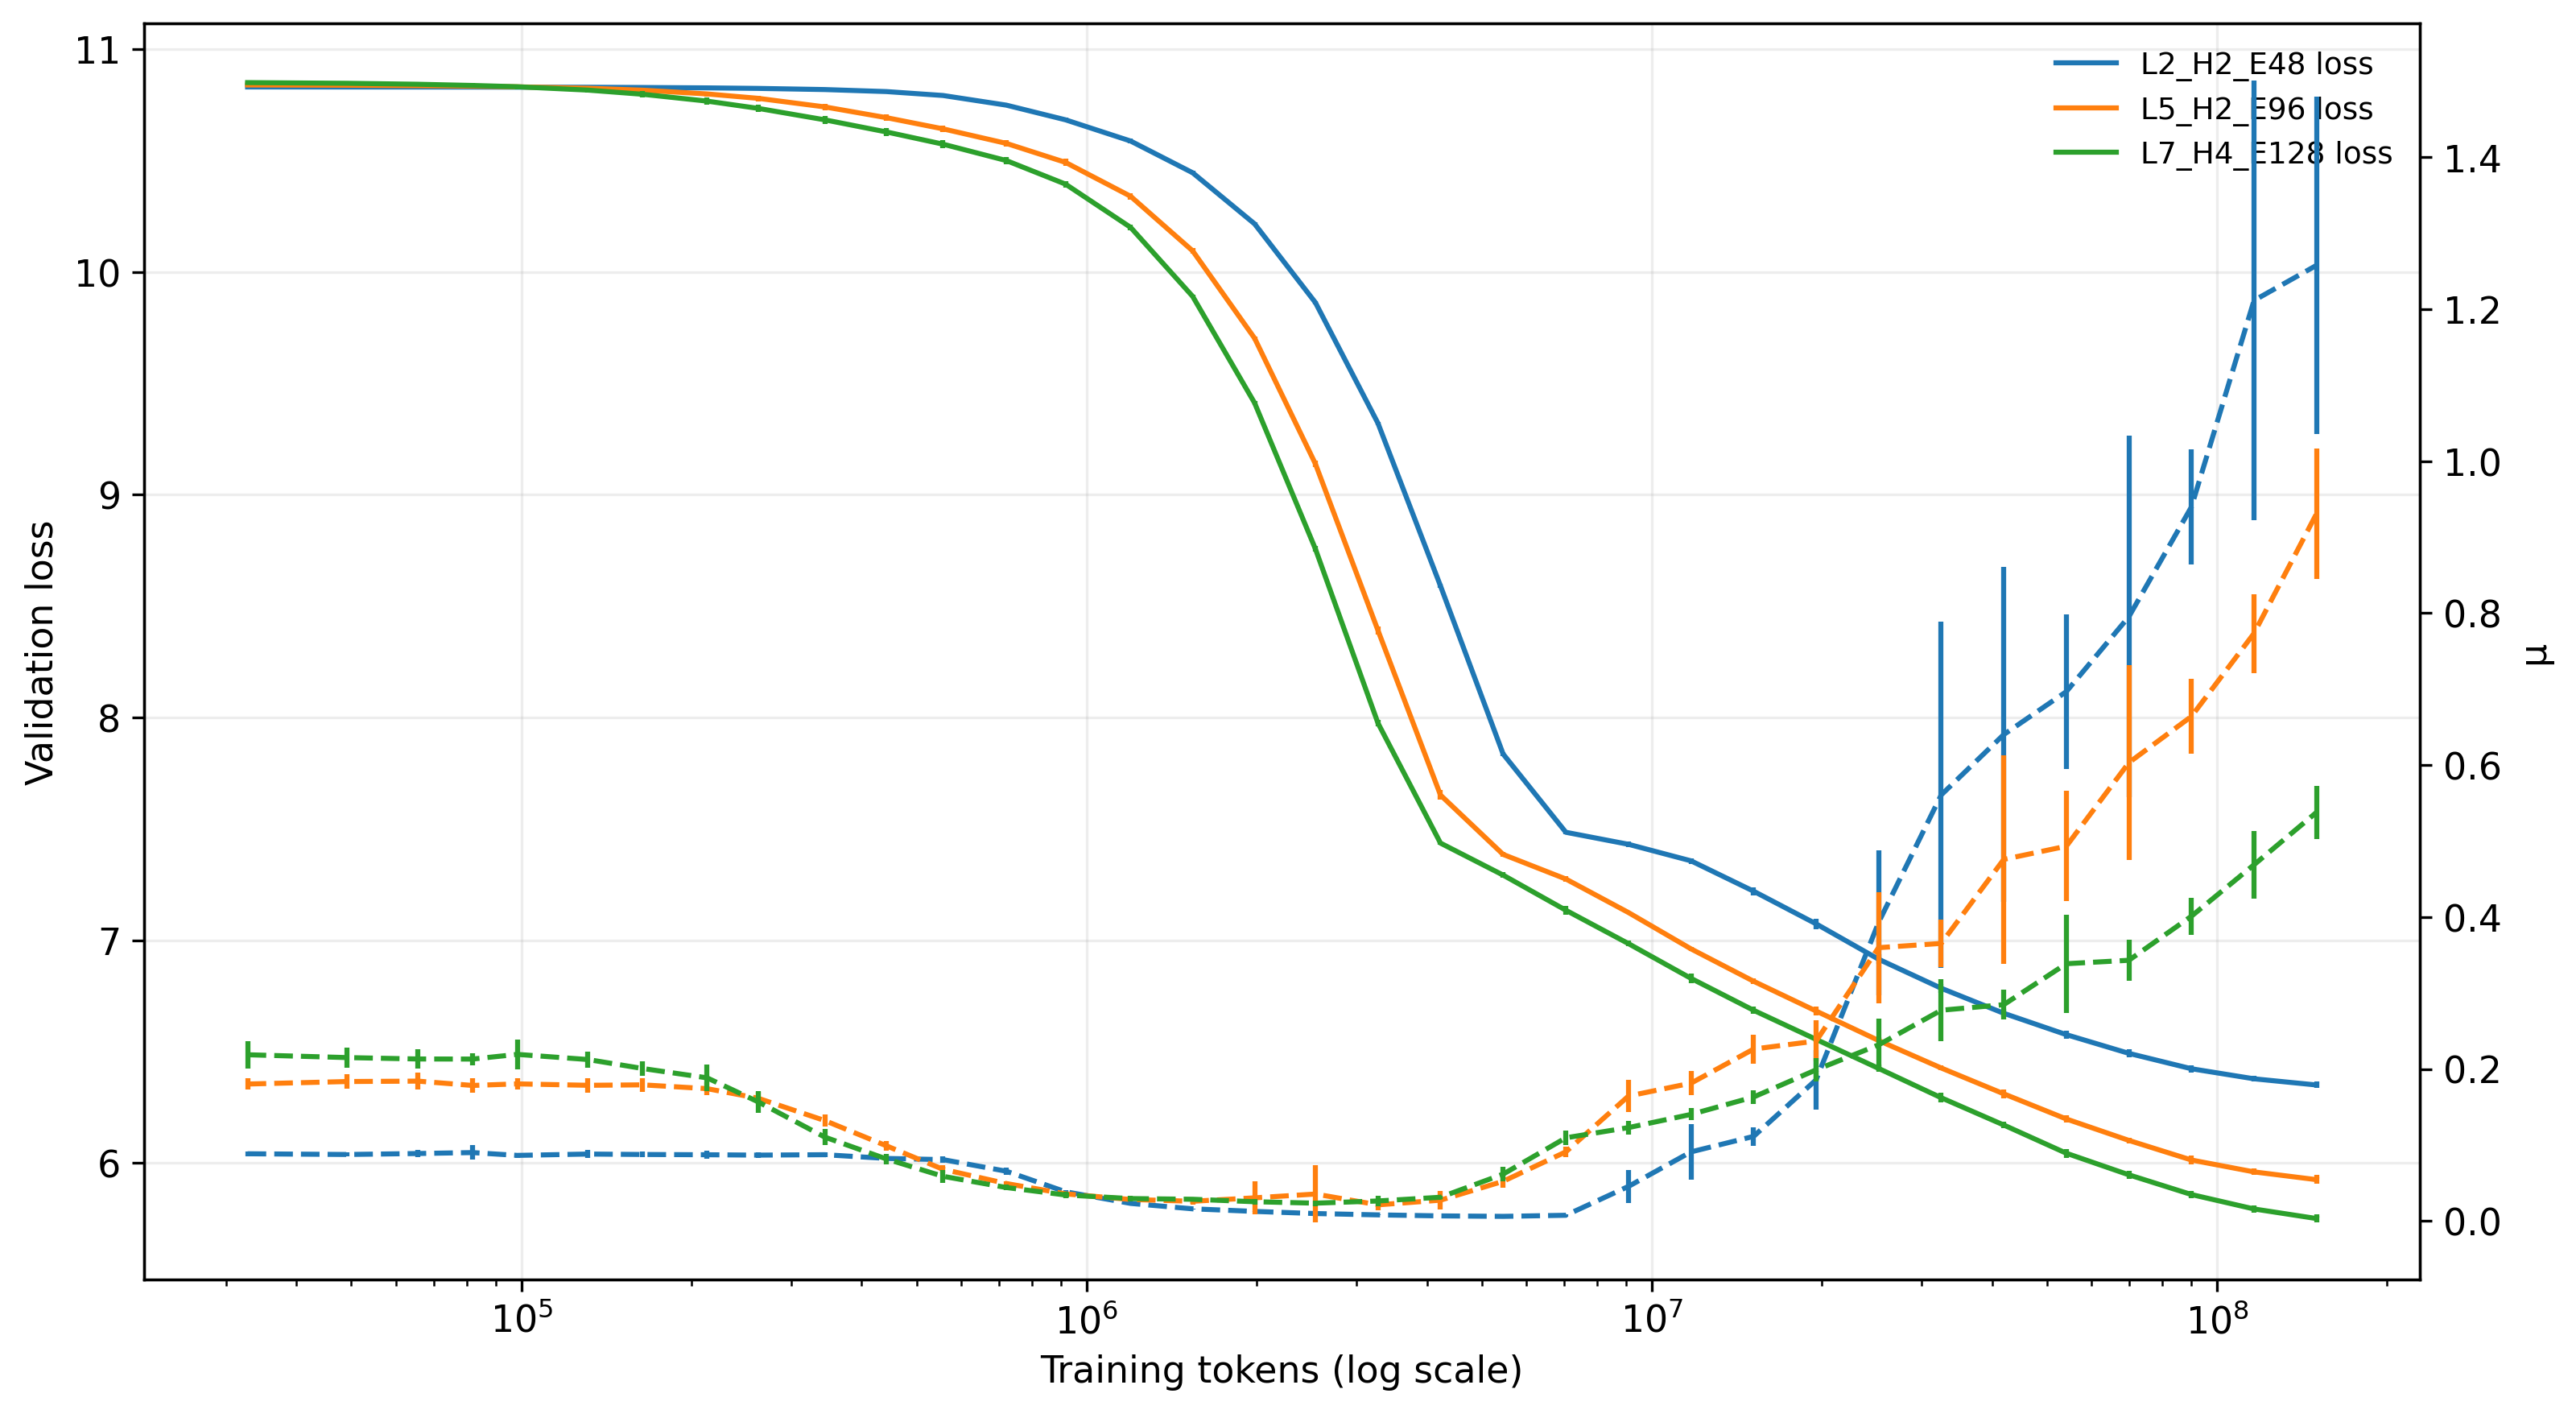
\includegraphics[width=0.92\linewidth]{fig_few_models_dynamics.png}
\caption{Для трех архитектур на одном графике показаны валидационная ошибка сплошной линией и ландшафтная мера пунктиром по числу обработанных токенов}
\label{fig:dynamics-anchor}
\end{figure}
\begin{figure}[ht]
\centering
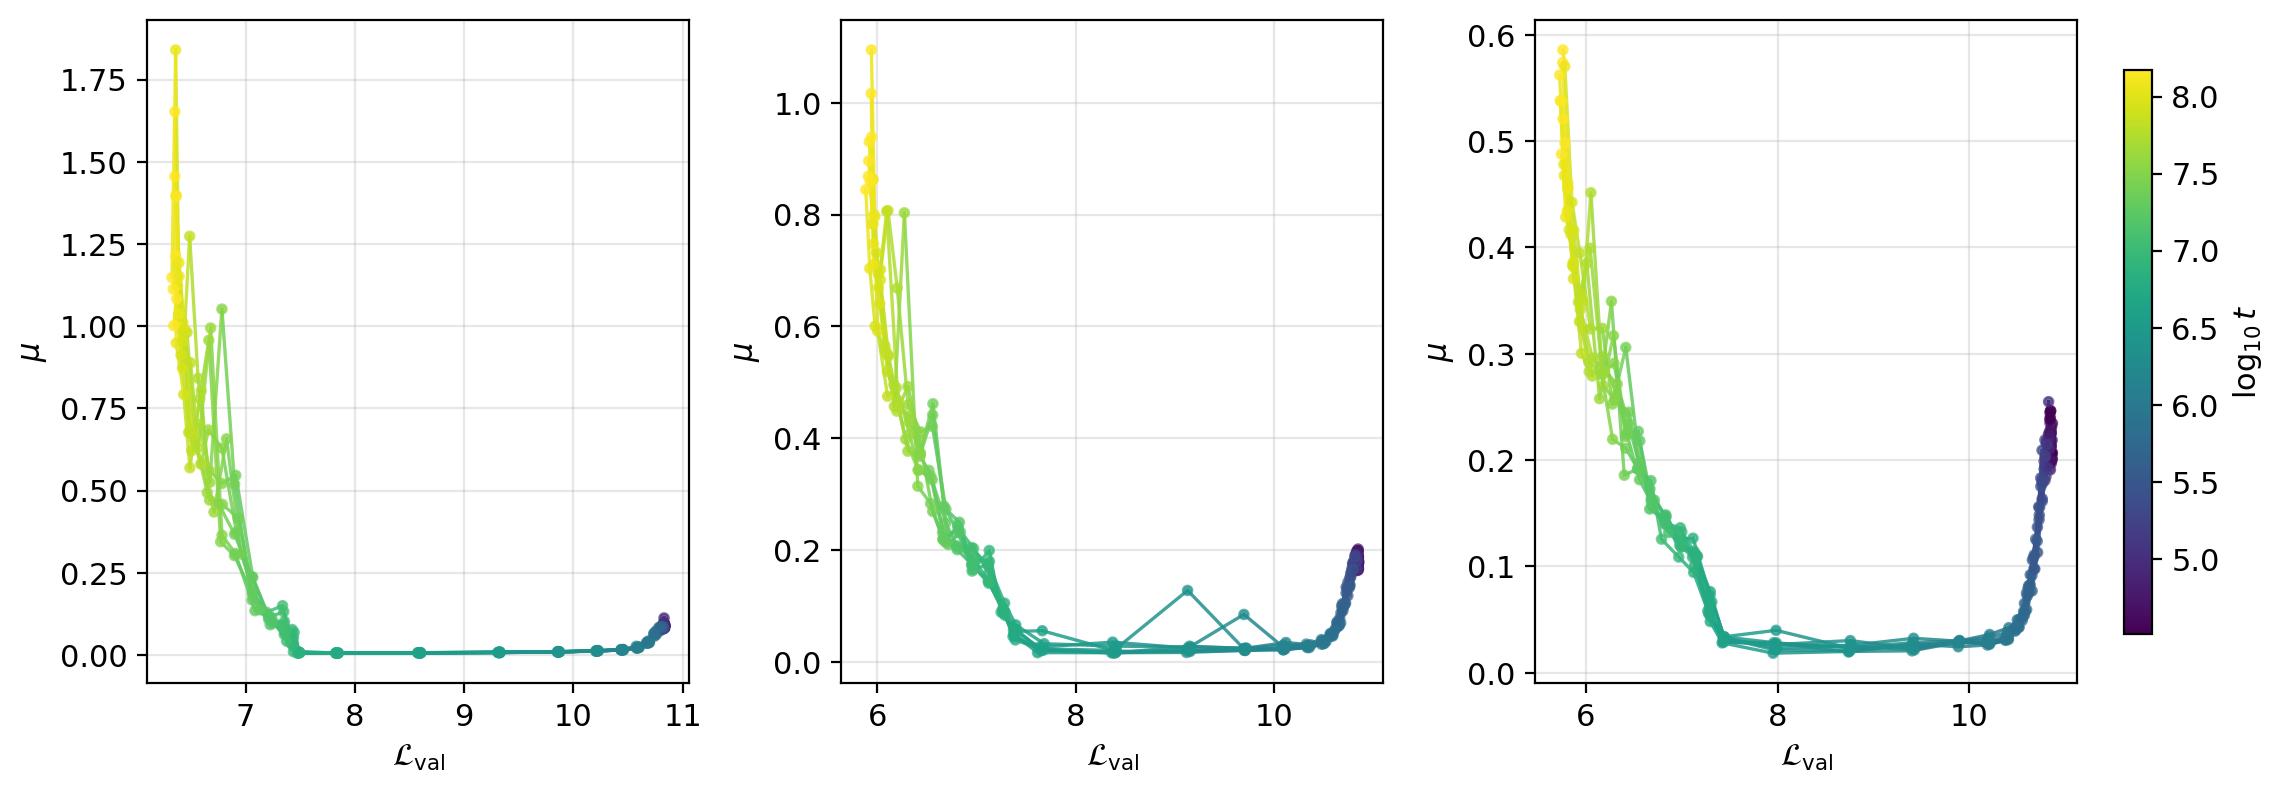
\includegraphics[width=0.98\linewidth]{fig_mu_val_phase_plane.png}
\caption{Зависимость между валидационной ошибкой и ландшафтной мерой для выборочных архитектур}
\label{fig:phase-plane}
\end{figure}
\begin{figure}[ht]
\centering
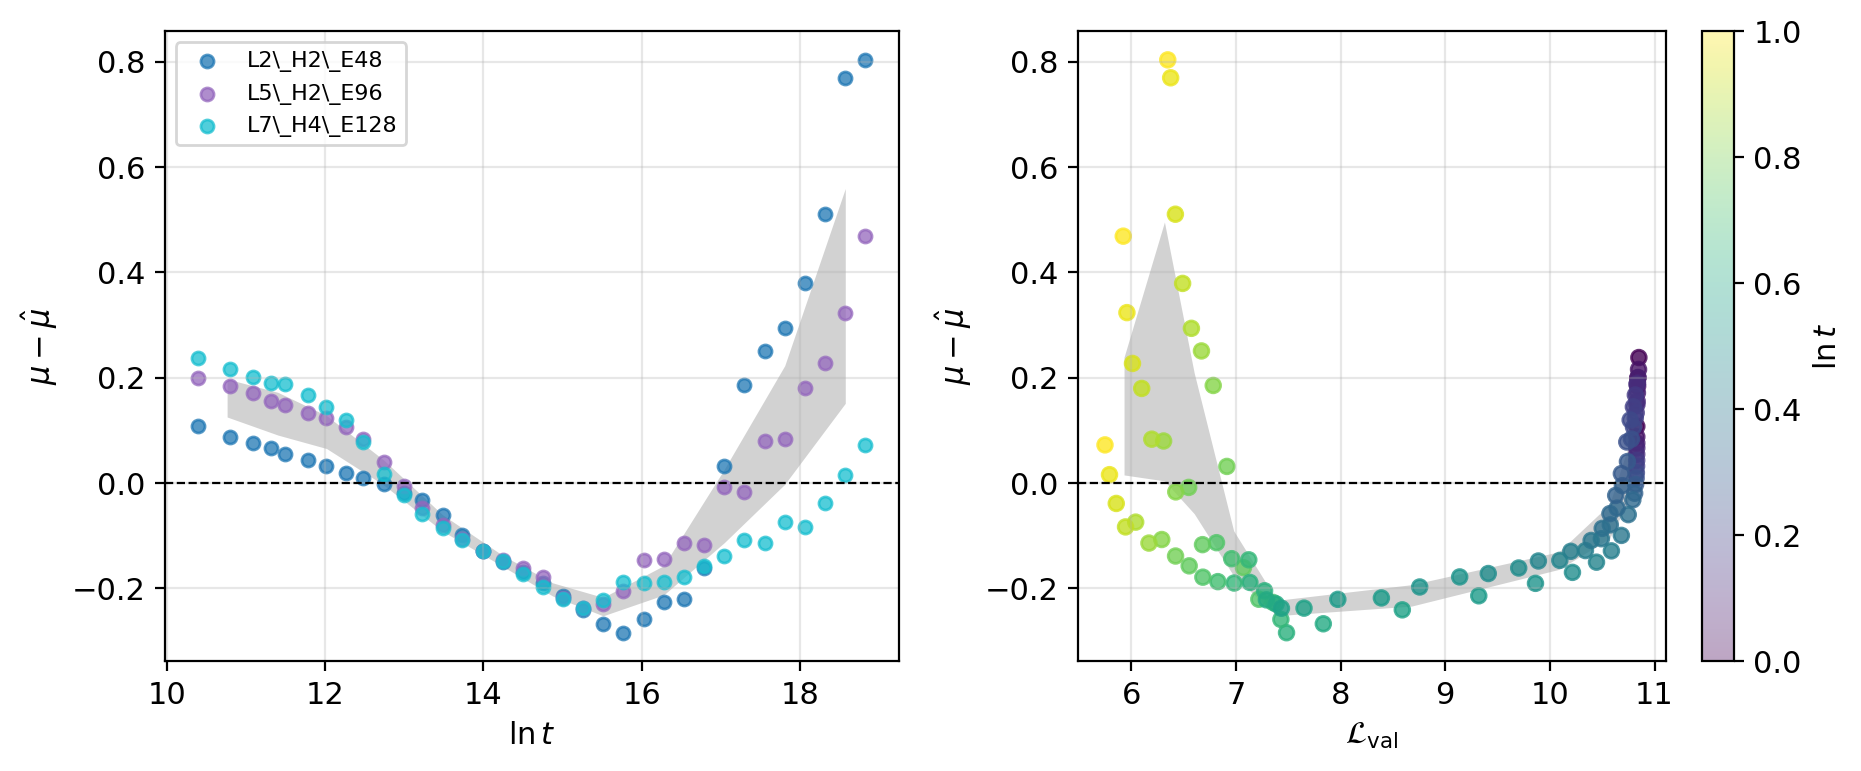
\includegraphics[width=0.98\linewidth]{fig_mu_residual_vs_loss_time.png}
\caption{Отклонение наблюдаемой ландшафтной меры от значения, предсказанного линейной моделью по валидационной ошибке и логарифму числа обучающих токенов}
\label{fig:mu-residual}
\end{figure}
\begin{figure}[ht]
\centering
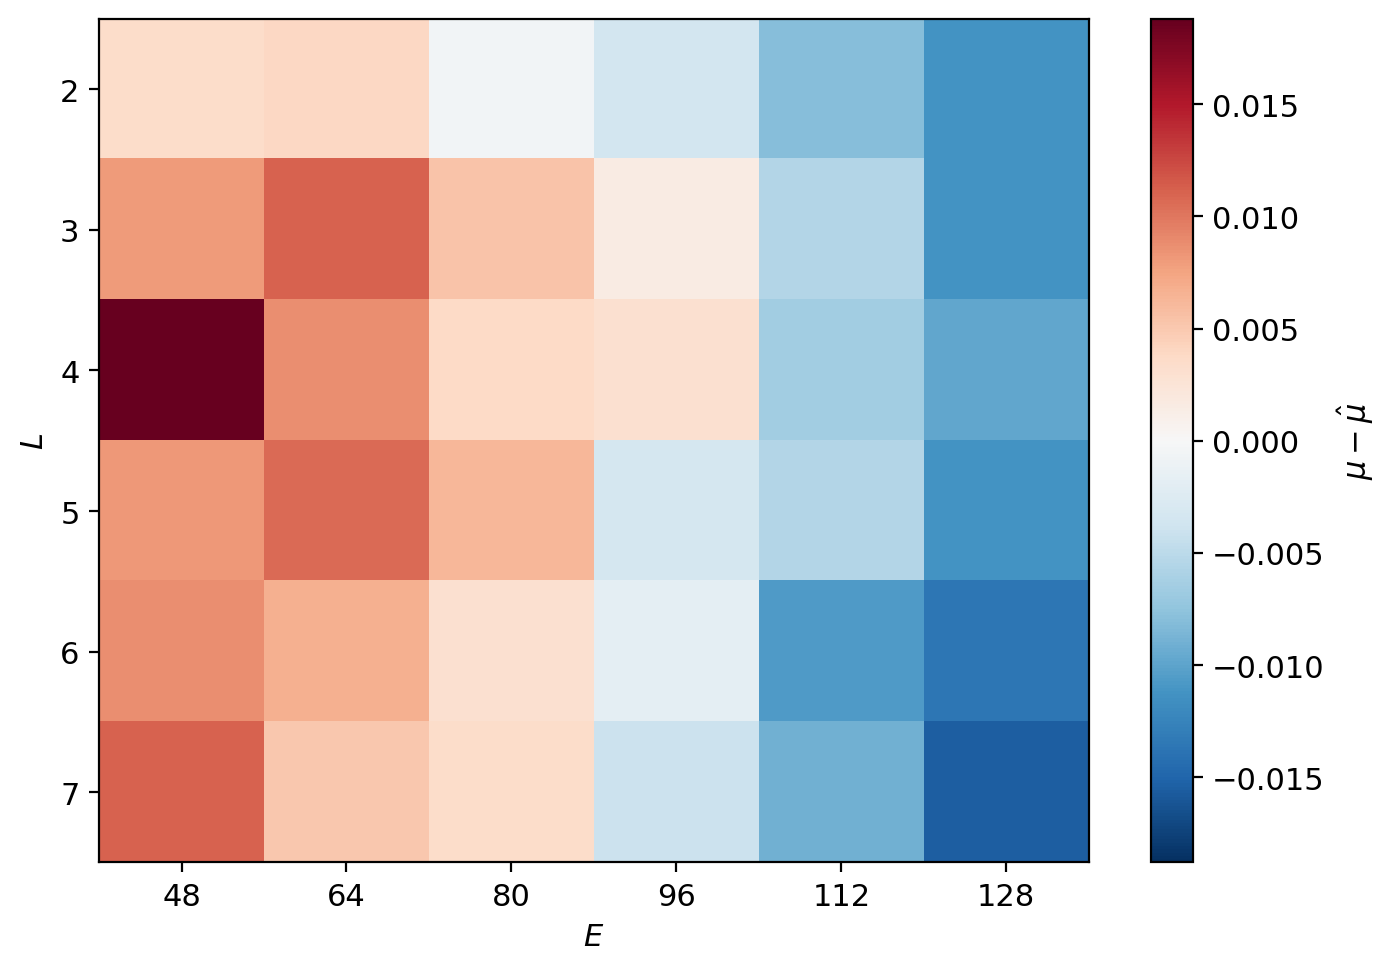
\includegraphics[width=0.92\linewidth]{fig_grid_mu_residual_heatmap.png}
\caption{Отклонения меры от линейной модели, после усреднения по восьми независимым запускам в каждой ячейке}
\label{fig:grid-residual-heatmap}
\end{figure}
\begin{figure}[ht]
\centering
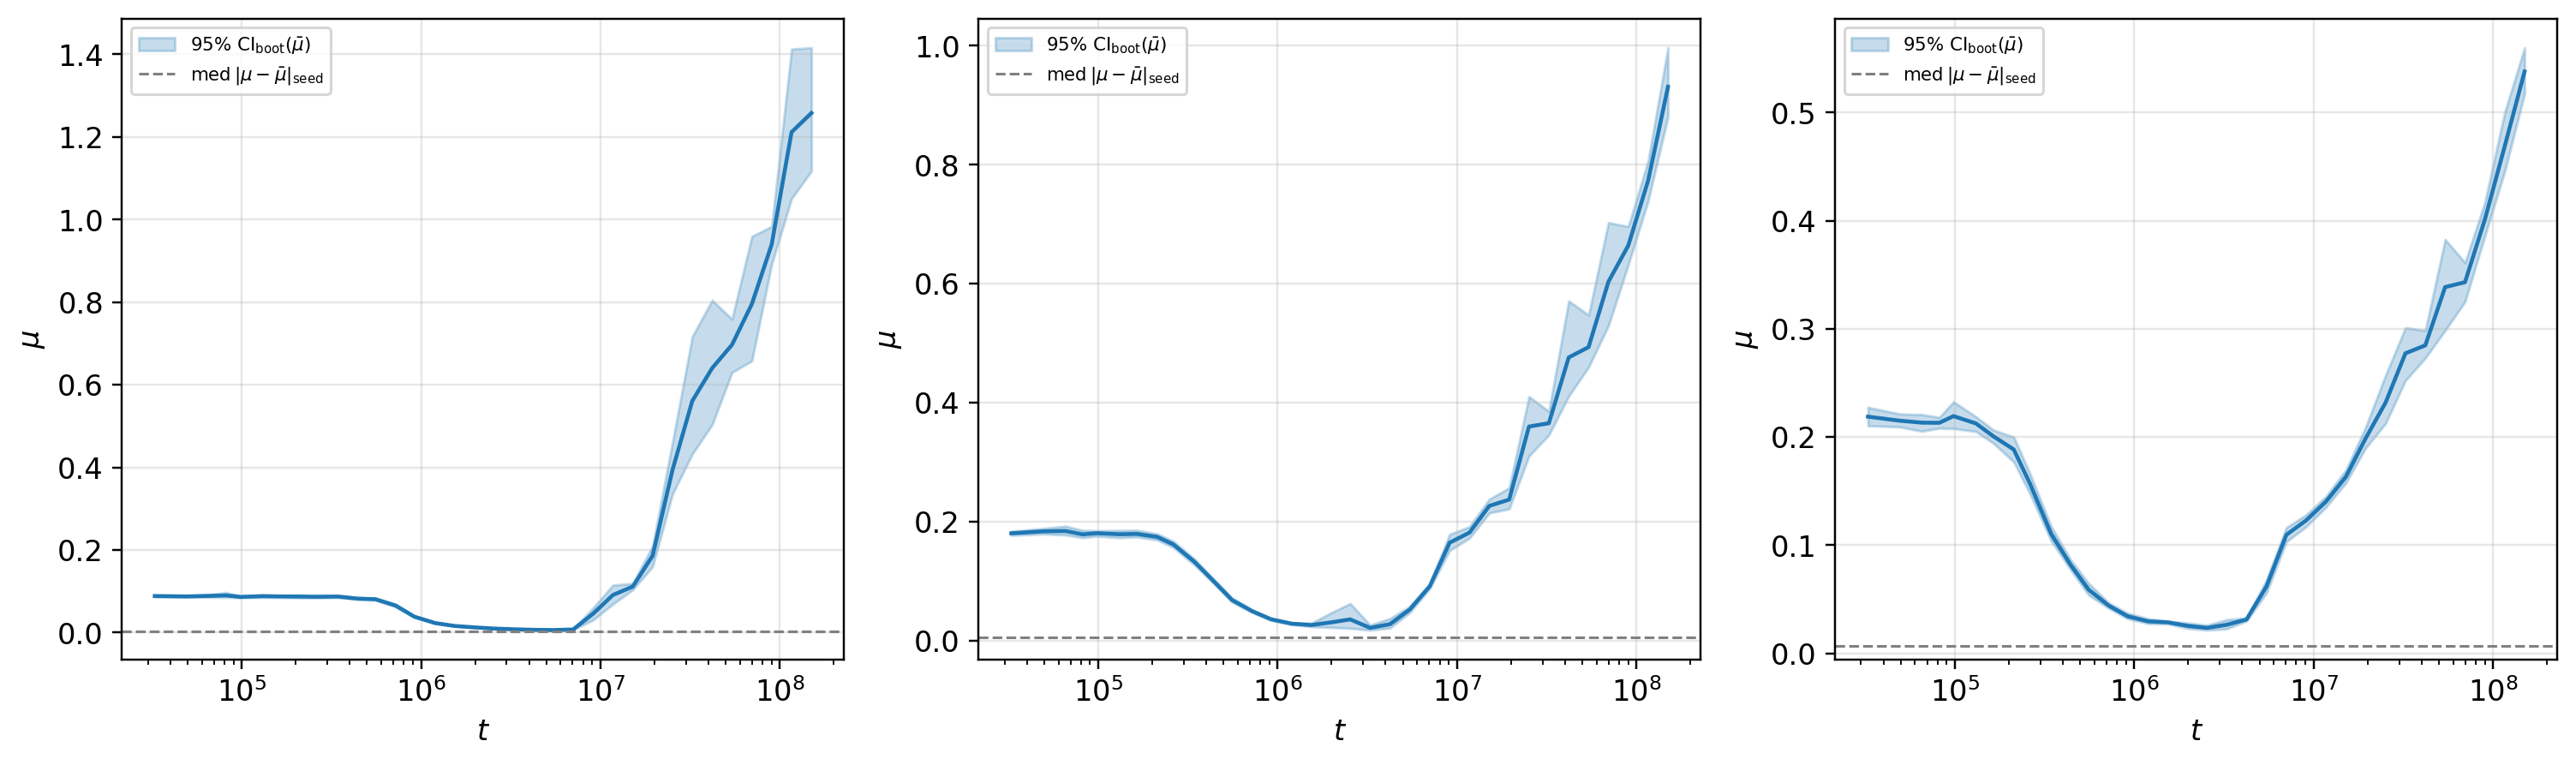
\includegraphics[width=0.98\linewidth]{fig_mu_seed_dispersion.png}
\caption{Выборочное среднее~$\mu$ по восьми независимым запускам}
\label{fig:mu-runs-disp}
\end{figure}
\begin{figure}[ht]
\centering
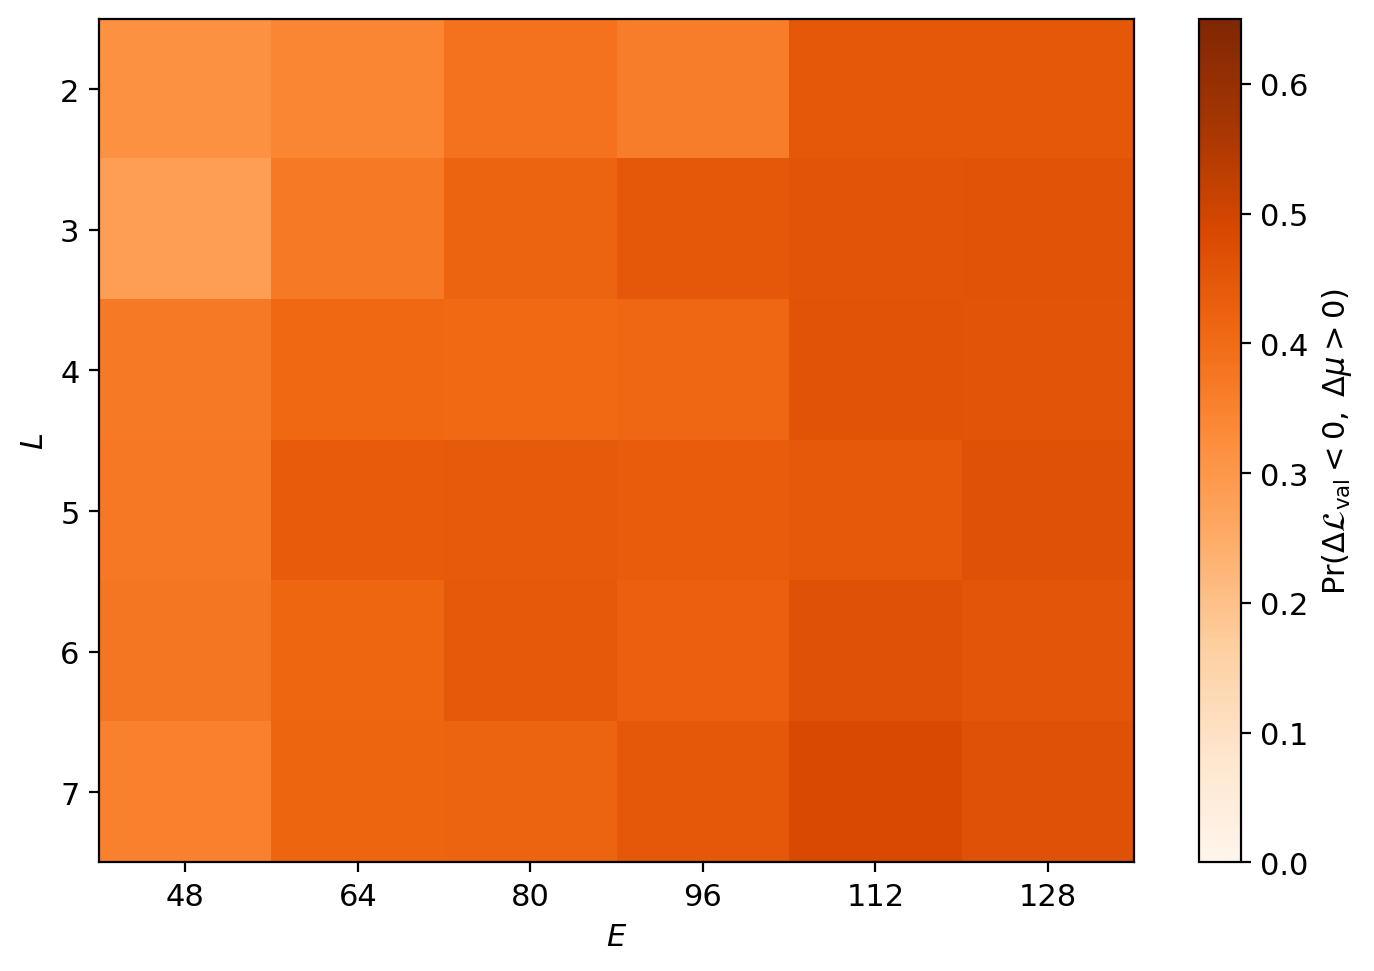
\includegraphics[width=0.88\linewidth]{fig_grid_nonmonotonicity_heatmap.png}
\caption{Доля последовательных пар контрольных точек с~$\Delta\mathcal{L}_{\mathrm{val}}<0$ и~$\Delta\mu>0$ по ячейкам~$(L,E)$ первой части эксперимента}
\label{fig:grid-nonmono}
\end{figure}
\begin{figure}[ht]
\centering
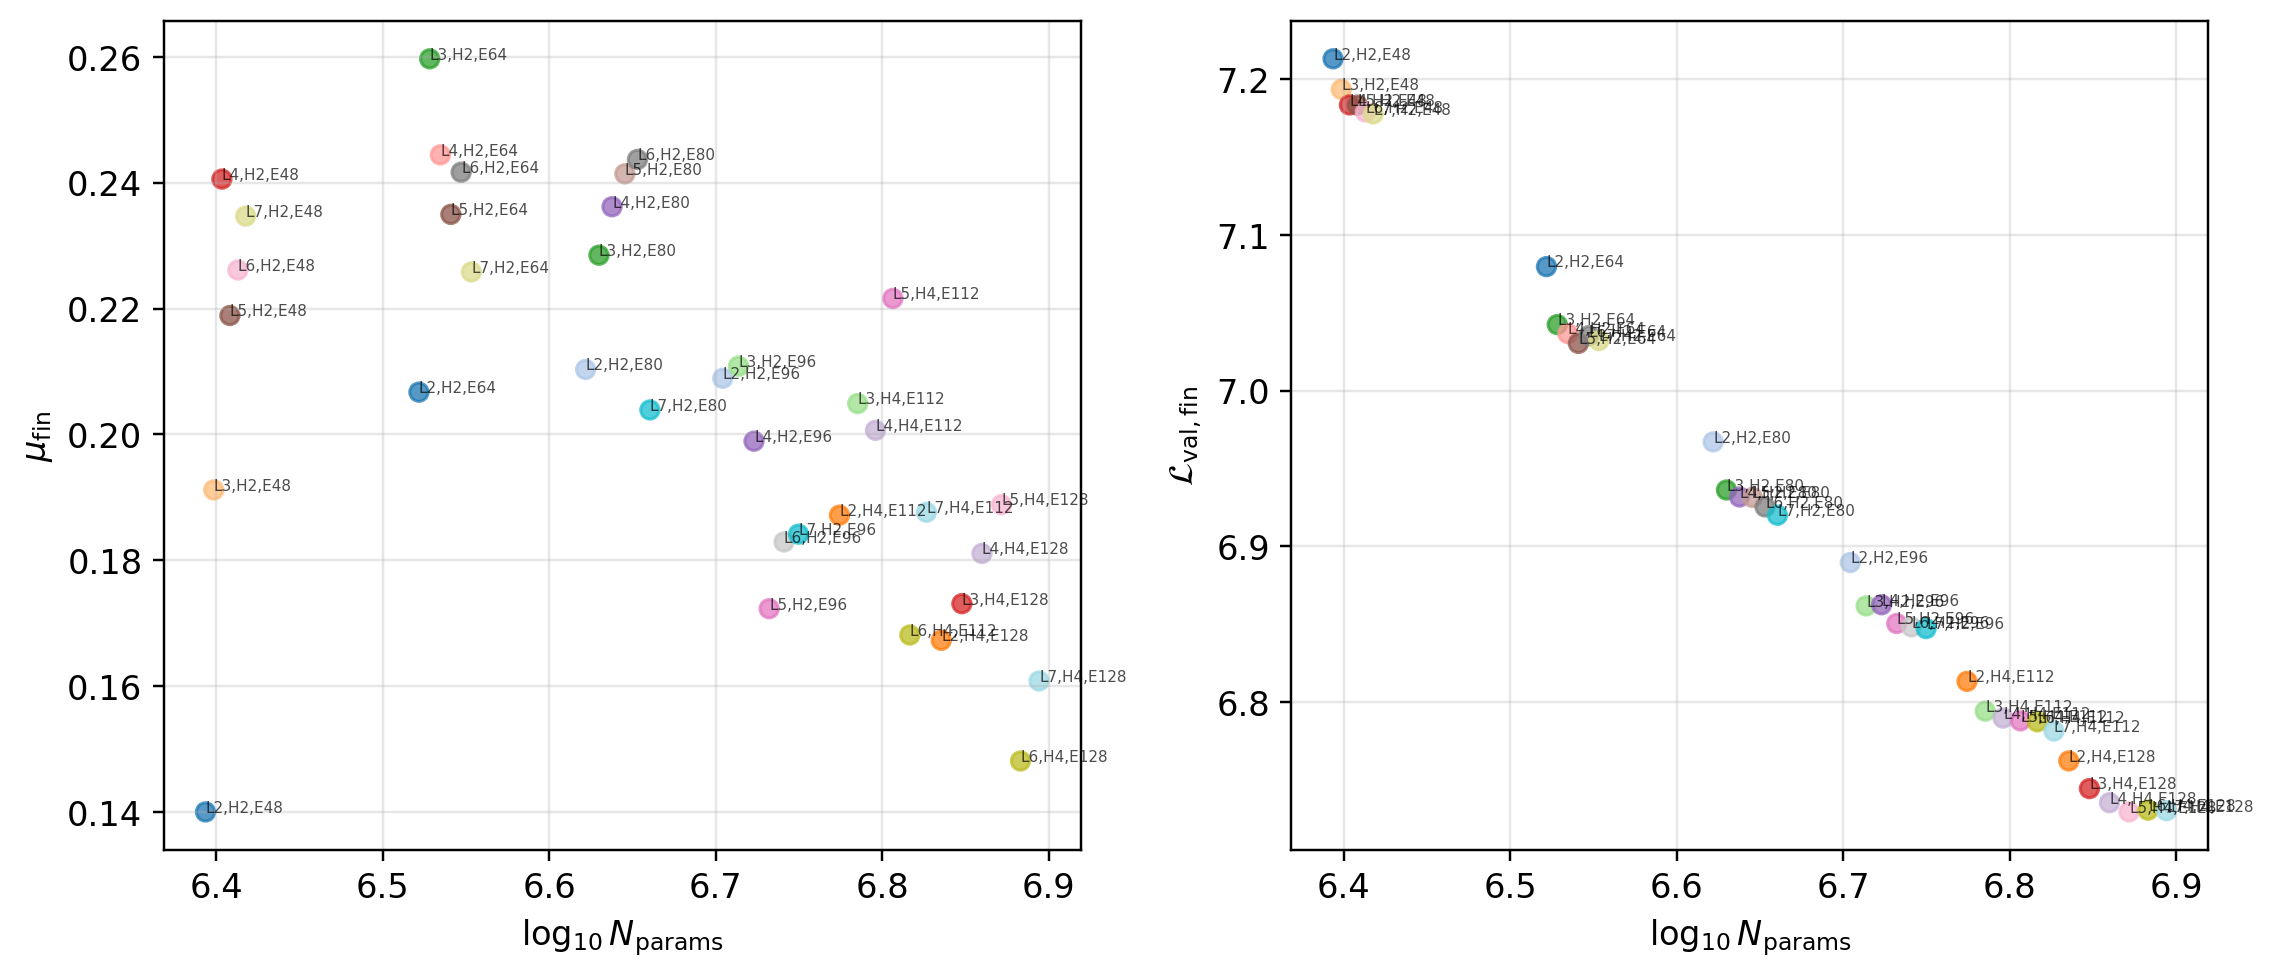
\includegraphics[width=0.98\linewidth]{fig_mu_arch_summary.png}
\caption{Финальная контрольная точка первой части эксперимента:~$\mu$ и~$\mathcal{L}_{\mathrm{val}}$ против десятичного логарифма числа обучаемых параметров~$N_{\mathrm{params}}$ для~$36$ архитектур}
\label{fig:arch-summary}
\end{figure}
\begin{figure}[ht]
\centering
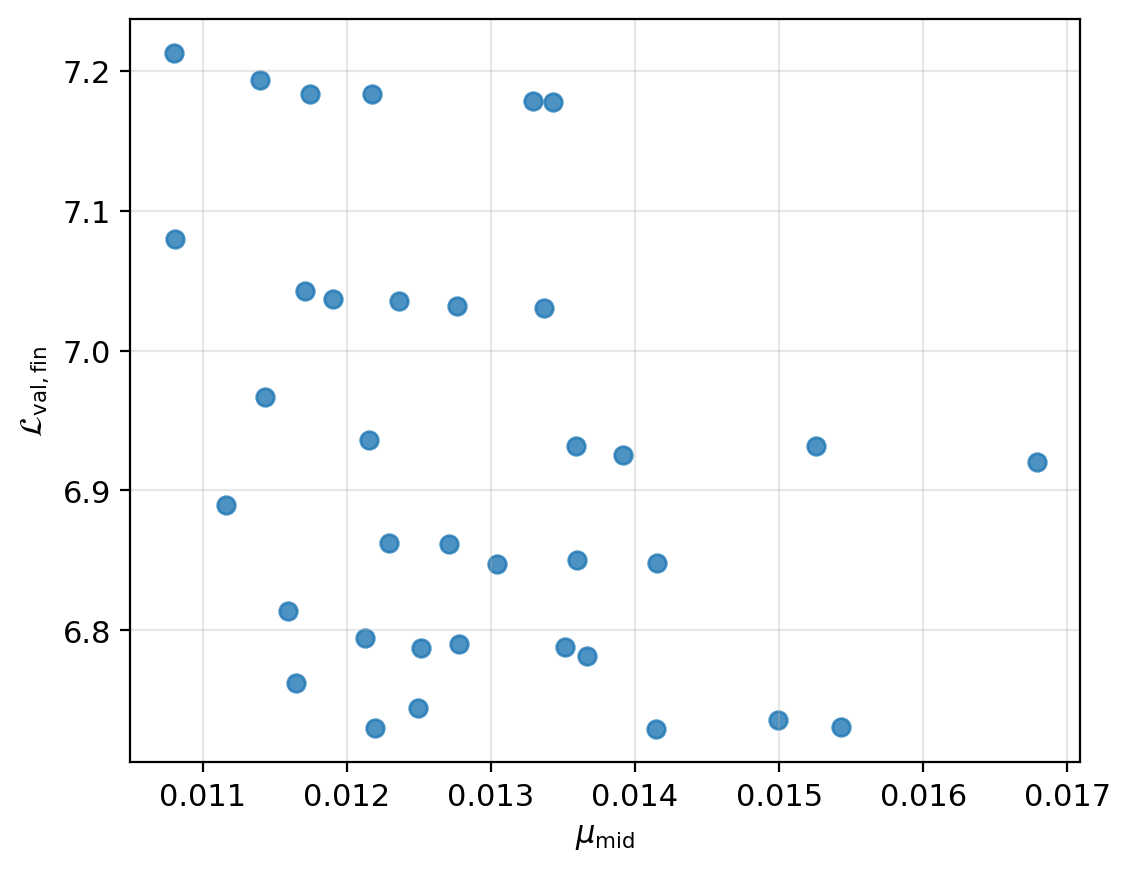
\includegraphics[width=0.72\linewidth]{fig_mu_mid_vs_val_final.png}
\caption{Выборочное среднее~$\mu$ по восьми запускам на контрольной точке с индексом, близким к медиане по сетке, и финальная валидационная ошибка по архитектурам первой части эксперимента}
\label{fig:mu-mid-valfinal}
\end{figure}

Для эмпирического анализа ландшафтной меры используется выборка WikiText-103~\cite{merity2016pointer}.
Токенизация текста согласована с языковой моделью GPT-2~\cite{radford2019language}.
Гиперпараметры архитектур для сравнения приведены в табл.~\ref{tab:arch-grid}.

В рамках вычислительного эксперимента спектральная норма разности~$\mathbf{H}_i-\bar{\mathbf{H}}$ не считается явно. Для каждого~$i$ задается семейство из~$r$ независимых случайных направлений~$v_j\in\mathbb{R}^d$,~$\|v_j\|_2=1$,~$j=1,\ldots,r$.
Далее по полному вектору обучаемых параметров производится вычисление гессиан-векторных произведений и величин~$\|(\mathbf{H}_i-\bar{\mathbf{H}})v_j\|_2$ без диагональной аппроксимации и без ограничения подмножества параметров.
Оценкой нормы разности служит максимум нормы по~$j$-му направлению.
При фиксированном наборе~$\{v_j\}$ это дает нижнюю оценку спектральной нормы, причем при каждом вычислении~$\mu$ выполняется пересэмплирование направлений.
Численные значения~$m$ и~$r$ указаны в табл.~\ref{tab:exp-params}.

Эксперимент состоит из двух частей.
В обоих частях используется одинаковый корпус текстов, токенизатор, согласование~$H$ с шириной скрытого слоя, оптимизатор AdamW и правила вычисления~$\mathcal{L}_{\mathrm{val}}$ и~$\mu$.
Меняется состав архитектур, горизонт обучения по числу токенов и расписание скорости обучения (англ. learning rate).
В первой части проводится обучение всех конфигураций из табл.~\ref{tab:arch-grid}.
Во второй части~--- три выбранные конфигурации с увеличенным горизонтом обучения по числу токенов.
Для каждой архитектуры выполняется~$8$ независимых запусков обучения с различными инициализациями и порядком стохастических операций.
Во всех экспериментах для динамики по токенам показаны траектории выборочных средних и~$95\%$ доверительные интервалы для матожидания по запускам.

Устойчивость оценки~$\mu$ относительно шума приведена в табл.~\ref{tab:noise-floor}.
Расширенный регрессионный разбор линейных аппроксимаций для второй части эксперимента приведен в табл.~\ref{tab:reg-summary}--\ref{tab:reg-coefs}.
Базовую линейную регрессию~$\mu\approx a+b\,\mathcal{L}_{\mathrm{val}}+c\ln t$ по агрегированным точкам второй части эксперимента обозначим \emph{M0}, в свою очередь различные модификации \emph{M1}--\emph{M4} отличаются набором дополнительных признаков, что указано в табл.~\ref{tab:reg-summary}.

На рис.~\ref{fig:loss-all}, \ref{fig:mu-all} и~\ref{fig:dynamics-anchor} траектории~$\mathcal{L}_{\mathrm{val}}(\theta_t)$ и~$\mu(\theta_t)$ сопоставлены по оси накопленных токенов.
Также на графиках показаны~$95\%$ доверительные интервалы матожидания по распределению~$8$ независимых запусков на каждой контрольной точке.
В первой части эксперимента для всех конфигураций табл.~\ref{tab:arch-grid} при росте числа токенов~$\mathcal{L}_{\mathrm{val}}$ улучшается на фиксированной сетке контрольных значений~$t$.
Кривые~$\mu(\theta_t)$ при этом не повторяют форму кривых потерь, так как у части архитектур после начального участка $\mu$ возрастает на поздних отрезках горизонта.
Во второй части эксперимента для трех выбранных архитектур $\mu(\theta_t)$ не является монотонной функцией~$t$ там, где $\mathcal{L}_{\mathrm{val}}$ по контрольным точкам убывает.
По рис.~\ref{fig:mu-runs-disp} и табл.~\ref{tab:noise-floor} видно, что амплитуда этих изменений существенно превышает типичный межзапусковый разброс реализаций~$\mu$ на одной контрольной точке относительно их выборочного среднего.

На рис.~\ref{fig:phase-plane} показана зависимость в координатах~$(\mathcal{L}_{\mathrm{val}},\mu)$.
Из диаграммы следует, что одному и тому же интервалу значений~$\mathcal{L}_{\mathrm{val}}$ могут соответствовать разные~$\mu$, причем разброс зависит от числа обработанных токенов и от номера независимого запуска.
Отсюда следует эксперимент, в рамках которого анализируется можно ли основную закономерность описать простой совместной зависимостью~$\mu$ от ошибки на валидации и от времени обучения.

На каждой контрольной точке второй части эксперимента берется пара~$(\mathcal{L}_{\mathrm{val}},\mu)$ после усреднения по восьми запускам как выборочное приближение совместного матожидания.
По совокупности таких точек оценивается базовая регрессия~\emph{M0}, то есть~$\mu\approx a+b\,\mathcal{L}_{\mathrm{val}}+c\ln t$, а предсказание модели обозначается~$\hat{\mu}$.
На трех архитектурах согласование умеренное~$R^2\approx 0{,}35$.
Отдельная подгонка по каждой архитектуре дает заметно более высокие~$R^2$: порядка~$0{,}50$,~$0{,}43$ и~$0{,}24$.
Значит, простая общая линейная форма не улавливает различия между архитектурами и смешивает разные режимы траекторий.

Остатки~$\mu-\hat{\mu}$ у M0 систематически отличны от нуля, а следовательно одних координат~$\mathcal{L}_{\mathrm{val}}$ и~$\ln t$ недостаточно, чтобы описать наблюдаемую связь.
На рис.~\ref{fig:mu-residual} показано, как меняется средний остаток по квантильным ячейкам по~$\ln t$ и по~$\mathcal{L}_{\mathrm{val}}$ вместе с доверительными интервалами.

С помощью частных коэффициентов корреляции Пирсона изолируется вклад времени при фиксированной ошибке и вклад ошибки при фиксированном времени.
Точечные оценки составляют~$\rho(\mu,\ln t\mid\mathcal{L}_{\mathrm{val}})\approx 0{,}179$ при интервале~$[-0{,}020,\;0{,}351]$ и~$\rho(\mu,\mathcal{L}_{\mathrm{val}}\mid\ln t)\approx -0{,}058$ при интервале~$[-0{,}252,\;0{,}135]$.
Доверительный интервал для~$\rho(\mu,\ln t\mid\mathcal{L}_{\mathrm{val}})$ почти не пересекает ноль, тогда как интервал для~$\rho(\mu,\mathcal{L}_{\mathrm{val}}\mid\ln t)$ содержит ноль, что согласуется с тем, что модель M0 объясняет лишь часть разброса.

Далее сравниваются расширения M1--M4 из табл.~\ref{tab:reg-summary}--\ref{tab:reg-coefs}.
Через~$d$ обозначено число обучаемых параметров конфигурации, через~$n$~--- объем обучающей части корпуса в токенах на соответствующем этапе.
Добавление слагаемых~$\ln N_{\mathrm{params}}$ и~$\ln(d/n)$ почти не повышает~$R^2$ относительно M0.
Существенный выигрыш дает слагаемое~$\mathcal{L}_{\mathrm{val}}\cdot\ln t$, то есть требуется совместный учет ошибки и горизонта, а не только их аддитивное включение вместе с логарифмом времени.

Та же линейная зависимость проверяется на данных первой части эксперимента, чтобы сопоставить две части эксперимента между собой.
На рис.~\ref{fig:grid-residual-heatmap} показана тепловая карта остатков по ячейкам~$(L,E)$ при~$R^2\approx 0{,}267$.
Качество описания ниже, чем во второй части эксперимента, а профиль остатков по ячейкам неоднороден, то есть отклонения от линейной формы зависят от конфигурации.

Отдельный разрез~--- согласованность локальных изменений ошибки и меры вдоль одной траектории.
На рис.~\ref{fig:grid-nonmono} по ячейкам~$(L,E)$ показана доля последовательных пар контрольных точек, где одновременно~$\Delta\mathcal{L}_{\mathrm{val}}<0$ и~$\Delta\mu>0$.
В первой части эксперимента средняя доля таких пар по траекториям составляет около~$41{,}5$\%, доверительные интервалы для среднего по траекториям равен~$[40{,}7,\;42{,}3]$\%.

На рисунках~\ref{fig:arch-summary} и~\ref{fig:mu-mid-valfinal} представлена связь финальных значений ошибки и~$\mu$ с масштабом модели и соотношение значения~$\mu$ на контрольной точке с почти медианным индексом по горизонту сетки с финальной ошибкой на том же этапе.

\section{Обсуждение}

\begin{table}[htbp]
\centering
\caption{Устойчивость оценки~$\mu$}
\label{tab:noise-floor}
\footnotesize
\setlength{\tabcolsep}{3pt}
\begin{tabularx}{\linewidth}{|>{\raggedright\arraybackslash}X|c|c|c|c|}
\hline
Конфигурация & med.\,std & размах & SNR & доля \\
\hline
L2\_H2\_E48 & $0.00406$ & $1.25169$ & $308.27$ & $66.7\%$ \\
L5\_H2\_E96 & $0.00949$ & $0.90973$ & $95.87$ & $72.2\%$ \\
L7\_H4\_E128 & $0.01058$ & $0.51444$ & $48.63$ & $75.0\%$ \\
Первая часть, медиана по 36 архитектурам & $0.00462$ & $0.19821$ & $43.17$ & $90.0\%$ \\
\hline
\end{tabularx}
\end{table}

\begin{table}[htbp]
\centering
\caption{Линейные спецификации для~$\mu$}
\label{tab:reg-summary}
\footnotesize
\setlength{\tabcolsep}{3pt}
\begin{tabularx}{\linewidth}{|l|c|c|c|c|>{\raggedright\arraybackslash}X|}
\hline
Модель & $R^2$ & $\bar R^2$ & $F$ vs M0 & $p$ \\
\hline
M0 & $0.350$ & $0.330$ & -- & -- \\
M1 & $0.362$ & $0.335$ & $1.83$ & $1.79\cdot 10^{-1}$ \\
M2 & $0.777$ & $0.768$ & $188.38$ & $1.49\cdot 10^{-24}$ \\
M3 & $0.602$ & $0.585$ & $61.99$ & $4.71\cdot 10^{-12}$ \\
M4 & $0.362$ & $0.335$ & $1.83$ & $1.79\cdot 10^{-1}$ \\
\hline
\end{tabularx}
\end{table}

\begin{table}[htbp]
\centering
\caption{Доверительные интервалы коэффициентов}
\label{tab:reg-coefs}
\footnotesize
\setlength{\tabcolsep}{4pt}
\begin{tabularx}{\linewidth}{|>{\raggedright\arraybackslash}p{2.75cm}|>{\raggedright\arraybackslash}X|}
\hline
M0 $a$ & $-0.2991$ \; [$-1.6756,\;0.8722$] \\
M0 $b(\mathcal{L}_{\mathrm{val}})$ & $-0.0186$ \; [$-0.0698,\;0.0451$] \\
M0 $c(\ln t)$ & $0.0463$ \; [$-0.0037,\;0.1083$] \\
\hline
M1 $a$ & $0.8541$ \; [$-0.7184,\;2.3416$] \\
M1 $b(\mathcal{L}_{\mathrm{val}})$ & $-0.0305$ \; [$-0.0774,\;0.0294$] \\
M1 $c(\ln t)$ & $0.0373$ \; [$-0.0071,\;0.0895$] \\
M1 доп. & $-0.0596$ \; [$-0.1500,\;0.0242$] \\
\hline
M2 $a$ & $-9.4180$ \; [$-12.1149,\;-6.9555$] \\
M2 $b(\mathcal{L}_{\mathrm{val}})$ & $0.8868$ \; [$0.6819,\;1.1191$] \\
M2 $c(\ln t)$ & $0.5916$ \; [$0.4503,\;0.7454$] \\
M2 доп. & $-0.0550$ \; [$-0.0684,\;-0.0438$] \\
\hline
\end{tabularx}
\end{table}

Валидационная ошибка отражает качество предсказания на отложенной выборке.
Ландшафтная мера~$\mu$ отражает иное свойство геометрии риска, именно она агрегирует рассогласование индивидуальных гессианов по контекстам из~$D_{\mathrm{probe}}$ в текущей точке~$\theta_t$.
Отсюда следует, что совпадение или расхождение траекторий~$\mathcal{L}_{\mathrm{val}}$ и~$\mu$ не укладывается в простую шкалу ``хорошего'' или ``плохого'' обобщения.

Выбор спектральной нормы в~\eqref{eq:mu-def} согласован с этой ролью.
Она измеряет максимальное усиление по направлению и тем самым ориентируется на доминирующие ``острые'' сингулярные режимы локальной кривизны.
Норма Фробениуса усредняла бы вклад всех координат матрицы и менее прицельно отражала бы такие доминирующие направления.
Отдельная проверка чувствительности выводов к замене нормы в работе не проводилась.

Наблюдаемый рост~$\mu$ при продолжающемся улучшении~$\mathcal{L}_{\mathrm{val}}$ интерпретируется как сигнал о смене локального режима геометрии риска.
Такой рост мог бы соответствовать усилению кривизны по отдельным контекстам.
Он же может частично отражать рост разброса матриц~$\mathbf{H}_i$ при более стабильном среднем~$\bar{\mathbf{H}}$.
Оба механизма совместимы с представленными траекториями, но их разделение требует дополнительных диагностик, например сопоставления норм~$\mathbf{H}_i$ и норм отклонений~$\mathbf{H}_i-\bar{\mathbf{H}}$.

При оценке~$\mu$ стохастический вклад неизбежен, так как на каждой контрольной точке пересэмплируются и~$D_{\mathrm{probe}}$, и пробные направления.
Поэтому межзапусковый разброс реализаций~$\mu$ смешивает различие инициализаций с этой стохастикой оценивания.
Тем не менее по табл.~\ref{tab:noise-floor} видно, что размах траектории выборочного среднего~$\mu$ по токенам на порядки превышает медианное по контрольным точкам выборочное стандартное отклонение~$\mu$ между восьмью запусками.
Это наблюдается и во второй, и в типичной конфигурации первой части эксперимента.

С практической стороны~$\mu$ логично использовать как дополнительную координату мониторинга рядом с~$\mathcal{L}_{\mathrm{val}}$ и временем обучения.
Она стыкуется с фазовым представлением на рис.~\ref{fig:phase-plane} и с кросс-архитектурными диаграммами рассеяния рис.~\ref{fig:arch-summary}--\ref{fig:mu-mid-valfinal}.
При этом не формулируются прямые утверждения о раннем предсказании переобучения или о выборе архитектуры по одной лишь~$\mu$.
Фиксируется более узкий вывод, о том, что~$\mu$ содержит вариацию, которую не вытягивают простые линейные формы только по паре~$(\mathcal{L}_{\mathrm{val}},\ln t)$, что следует из регрессионного сравнения в табл.~\ref{tab:reg-summary}.

Также стоит отдельно отметить ограничесть данной работы.
Они касаются узкого семейства GPT-2 на WikiText-103 при фиксированном оптимизаторе AdamW, а следовательно перенос выводов на другие архитектуры, корпуса и масштабы остается открытым вопросом.
Сопоставление~$\mu$ со следом или спектральным радиусом агрегированного Гессиана, равно как и более богатые регрессионные модели, отнесены к дальнейшей работе.

\section{Выводы и перспективы}

В работе показано, что динамика $\mu$ в процессе обучения содержит дополнительную информацию о геометрическом режиме и не сводится к динамике валидационной функции потерь.
Этот вывод поддерживается согласованным анализом иллюстраций рис.~\ref{fig:loss-all}--\ref{fig:mu-residual}, тепловых карт рис.~\ref{fig:grid-residual-heatmap}--\ref{fig:grid-nonmono}, количественными данными табл.~\ref{tab:noise-floor} и расширенным регрессионным сравнением в табл.~\ref{tab:reg-summary}.
Результат согласуется с разделением ролей, где для опорной точки построены теоретические верхние оценки на~$\mu$, а в настоящей работе тот же показатель оценивается выборочно на пробной мини-выборке вдоль траектории обучения языковых моделей и используется для эмпирического сравнения архитектур.

Дальнейшая работа связана с расширением сетки архитектур и корпусов, увеличением числа независимых запусков обучения, прямым сопоставлением $\mu$ со следами и спектральными характеристиками агрегированного Гессиана, а также разработкой ускоренных спектральных приближений для оценки $\mu$ на больших моделях.

\begin{thebibliography}{99}

\bibitem{bartlett2002}
{\MakeUppercase{Bartlett~P.L., Mendelson~S.}}
\textit{Rademacher and Gaussian complexities: Risk bounds and structural results}~//
\emph{Journal of Machine Learning Research}.~-- 2002.~-- Vol.~3.~-- P.~463--482.

\bibitem{harvey2019jmlr}
{\MakeUppercase{Bartlett~P.L., Harvey~N., Liaw~C., Mehrabian~A.}}
\textit{Nearly-tight VC-dimension and pseudodimension bounds for piecewise linear neural networks}~//
\emph{Journal of Machine Learning Research}.~-- 2019.~-- Vol.~20, Paper~No.~63.~-- P.~1--17.

\bibitem{choromanska2015}
{\MakeUppercase{Choromanska~A., Henaff~M., Mathieu~M., Arous~G.B., LeCun~Y.}}
\textit{The loss surfaces of multilayer networks}~//
\emph{Proceedings of the 18th International Conference on Artificial Intelligence and Statistics (AISTATS)}, JMLR Workshop and Conference Proceedings, Vol.~38.~-- 2015.~-- P.~192--204.

\bibitem{dinh2017sharp}
{\MakeUppercase{Dinh~L., Pascanu~R., Bengio~S., Bengio~Y.}}
\textit{Sharp minima can generalize for deep nets}~//
\emph{Proceedings of the 34th International Conference on Machine Learning (ICML)}.~-- 2017.~-- P.~1019--1028.

\bibitem{fort2019emergent}
{\MakeUppercase{Fort~S., Ganguli~S.}}
\textit{Emergent properties of the local geometry of neural loss landscapes}~//
\emph{arXiv preprint arXiv:1910.05929}.~-- 2019.

\bibitem{fort2019large}
{\MakeUppercase{Fort~S., Jastrzebski~S.}}
\textit{Large scale structure of neural network loss landscapes}~//
\emph{Advances in Neural Information Processing Systems 33 (NeurIPS 2019)}.~-- 2019.

\bibitem{ghorbani2019}
{\MakeUppercase{Ghorbani~B., Krishnan~S., Xiao~Y.}}
\textit{An Investigation into Neural Net Optimization via Hessian Eigenvalue Density}~//
\emph{Proceedings of the 36th International Conference on Machine Learning}, PMLR~97.~-- 2019.~-- P.~2232--2241.


\bibitem{hochreiter1994}
{\MakeUppercase{Hochreiter~S., Schmidhuber~J.}}
\textit{Simplifying neural nets by discovering flat minima}~//
\emph{Advances in Neural Information Processing Systems 7 (NIPS 1994)}.~-- 1994.~-- P.~529--536.

\bibitem{hoffmann2022}
{\MakeUppercase{Hoffmann~J., Borgeaud~S., Mensch~A.~et~al.}}
\textit{An empirical analysis of compute-optimal large language model training}~//
\emph{Advances in Neural Information Processing Systems 35 (NeurIPS 2022)}.~-- 2022.

\bibitem{jacot2018ntk}
{\MakeUppercase{Jacot~A., Gabriel~F., Hongler~C.}}
\textit{Neural tangent kernel: Convergence and generalization in neural networks}~//
\emph{Advances in Neural Information Processing Systems 32 (NeurIPS 2018)}.~-- 2018.

\bibitem{kaplan2020}
{\MakeUppercase{Kaplan~J., McCandlish~S., Henighan~T.~et~al.}}
\textit{Scaling laws for neural language models}~//
\emph{arXiv preprint arXiv:2001.08361}.~-- 2020.

\bibitem{kiselev2024}
{\MakeUppercase{Kiselev~N.S., Grabovoy~A.V.}}
\textit{Unraveling the Hessian: A key to smooth convergence in loss function landscapes}~//
\emph{Doklady Mathematics}.~-- 2024.~-- Vol.~110 (Suppl.~2).~-- P.~S49--S61.

\bibitem{lee2018wide}
{\MakeUppercase{Lee~J., Xiao~L., Schoenholz~S.S., Bahri~Y., Novak~R., Sohl-Dickstein~J., Pennington~J.}}
\textit{Wide neural networks of any depth evolve as linear models under gradient descent}~//
\emph{Advances in Neural Information Processing Systems 33 (NeurIPS 2019)}.~-- 2019.

\bibitem{li2018visualizing}
{\MakeUppercase{Li~H., Xu~Z., Taylor~G., Studer~C., Goldstein~T.}}
\textit{Visualizing the loss landscape of neural nets}~//
\emph{Advances in Neural Information Processing Systems 32 (NeurIPS 2018)}.~-- 2018.

\bibitem{merity2016pointer}
{\MakeUppercase{Merity~S., Xiong~C., Bradbury~J., Socher~R.}}
\textit{Pointer sentinel mixture models}~//
\emph{arXiv preprint arXiv:1609.07843}.~-- 2016.

\bibitem{meshkov2024ispras}
{\MakeUppercase{Meshkov~V.Yu., Kiselev~N.S., Grabovoy~A.V.}}
\textit{ConvNets landscape convergence: Hessian-based analysis of matricized networks}~//
\emph{Proceedings of the 2024 Ivannikov ISP RAS Open Conference (ISPRAS)}.~-- IEEE, 2024.

\bibitem{neyshabur2017exploring}
{\MakeUppercase{Neyshabur~B., Bhojanapalli~S., McAllester~D., Srebro~N.}}
\textit{Exploring generalization in deep learning}~//
\emph{Advances in Neural Information Processing Systems 31 (NeurIPS 2017)}.~-- 2017.

\bibitem{papyan2019}
{\MakeUppercase{Papyan~V.}}
\textit{Measurements of Three-Level Hierarchical Structure in the Outliers in the Spectrum of Deepnet Hessians}~//
\emph{Proceedings of the 36th International Conference on Machine Learning}, PMLR~97.~-- 2019.~-- P.~5012--5021.

\bibitem{pennington2017}
{\MakeUppercase{Pennington~J., Bahri~Y.}}
\textit{Geometry of neural network loss surfaces via random matrix theory}~//
\emph{Proceedings of the 34th International Conference on Machine Learning (ICML)}.~-- 2017.~-- P.~2798--2806.

\bibitem{petrov2025curvaturegap}
{\MakeUppercase{Petrov~E., Kiselev~N., Meshkov~V., Grabovoy~A.}}
\textit{Closing the curvature gap: full transformer Hessians and their implications for scaling laws}~//
\emph{arXiv preprint arXiv:2510.16927}.~-- 2025.

\bibitem{radford2019language}
{\MakeUppercase{Radford~A., Wu~J., Child~R., Luan~D., Amodei~D., Sutskever~I.}}
\textit{Language models are unsupervised multitask learners}~//
OpenAI technical report.~-- 2019.

\bibitem{sagun2018}
{\MakeUppercase{Sagun~L., Evci~U., Guney~V.U., Dauphin~Y., Bottou~L.}}
\textit{Empirical analysis of the Hessian of over-parametrized neural networks}~//
\emph{arXiv preprint arXiv:1706.04454}.~-- 2017.

\bibitem{singh2022double}
{\MakeUppercase{Singh~S.P., Lucchi~A., Hofmann~T., Scholkopf~B.}}
\textit{Phenomenology of double descent in finite-width neural networks}~//
\emph{International Conference on Learning Representations (ICLR)}.~-- 2022.

\bibitem{singh2024lmc}
{\MakeUppercase{Singh~S.P., Adilova~L., Kamp~M., Fischer~A., Scholkopf~B., Hofmann~T.}}
\textit{Landscaping linear mode connectivity}~//
\emph{arXiv preprint arXiv:2406.16300}.~-- 2024.

\bibitem{tang2025hessian}
{\MakeUppercase{Tang~Q.-Y., Gu~Y., Cai~Y., Sun~M., Li~P., Xun~Z., Xie~Z.}}
\textit{Investigating the Overlooked Hessian Structure: From CNNs to LLMs}~//
\emph{Proceedings of the 42nd International Conference on Machine Learning (ICML)}, PMLR~267.~-- 2025.~-- P.~58805--58831.

\bibitem{vapnik1998}
{\MakeUppercase{Vapnik~V.N.}}
\textit{Statistical Learning Theory}.~-- New~York: Wiley, 1998.~-- 736~p.

\bibitem{wu2022dissecting}
{\MakeUppercase{Wu~Y., Zhu~X., Wu~C., Wang~A., Ge~R.}}
\textit{Dissecting Hessian: Understanding common structure of Hessian in neural networks}~//
\emph{arXiv preprint arXiv:2010.04261}.~-- 2020.

\end{thebibliography}

\makeenginfo
\makeauxinfo

\end{document}